\documentclass[10pt, xcolor=x11names,compress]{beamer}
\usepackage{tabulary}
\usepackage{booktabs}
\usepackage{float}
\usepackage{graphicx}
\usepackage{mwe}% for example pictures
\usepackage{siunitx}
\usepackage{hyperref}

\definecolor{sangria}{rgb}{0.57, 0.0, 0.04}
\usecolortheme[named=sangria]{structure}
\useoutertheme{infolines}
\usefonttheme[onlymath]{serif}
\setbeamertemplate{headline}[default]
\setbeamertemplate{navigation symbols}{}
\mode<beamer>{\setbeamertemplate{blocks}[rounded][shadow=true]}
\setbeamercovered{transparent}
\setbeamercolor{block body}{use=structure, fg=white, bg=black!20}
\setbeamercolor{itemize item}{fg=black}
\setbeamercolor{itemize subitem}{fg=gray} 
\setbeamercolor{itemize subsubitem}{fg=black!20} 
\makeatletter\setbeamertemplate{footline}
{  
	\leavevmode%  
	\hbox{%  
		\begin{beamercolorbox}[wd=.333333\paperwidth,ht=2.25ex,dp=1ex,center]{author in head/foot}%    
			\usebeamerfont{author in head/foot}
			\insertshortauthor%~~\beamer@ifempty{\insertshortinstitute}{}
		\end{beamercolorbox}%  
		\begin{beamercolorbox}[wd=.333333\paperwidth,ht=2.25ex,dp=1ex,center]{institute in head/foot}%    
			\usebeamerfont{title in head/foot}\insertinstitute  
		\end{beamercolorbox}%  
		\begin{beamercolorbox}[wd=.333333\paperwidth,ht=2.25ex,dp=1ex,right]{date in head/foot}%    
			\usebeamerfont{date in head/foot}\insertshortdate{}\hspace*{2em}    
			\insertframenumber{} / \inserttotalframenumber\hspace*{2ex}   
	\end{beamercolorbox}}%  
	\vskip0pt%
}
\makeatother 
\useoutertheme[footline=empty, subsection=false]{miniframes}
\usepackage{multicol}  
\author{Núcleo de Estudos Raciais}
\title{Apresentação - Resultados Preliminares Carta de Conjuntura Mercado de Trabalho}

\institute{Insper}\date{10/07/2024} 
\begin{document}
	\begin{frame}
		\titlepage
	\end{frame}
	
	
	\section{Estatística Descritiva} 
	\begin{frame}{População Economicamente Ativa}
		\begin{figure}
			\centering
			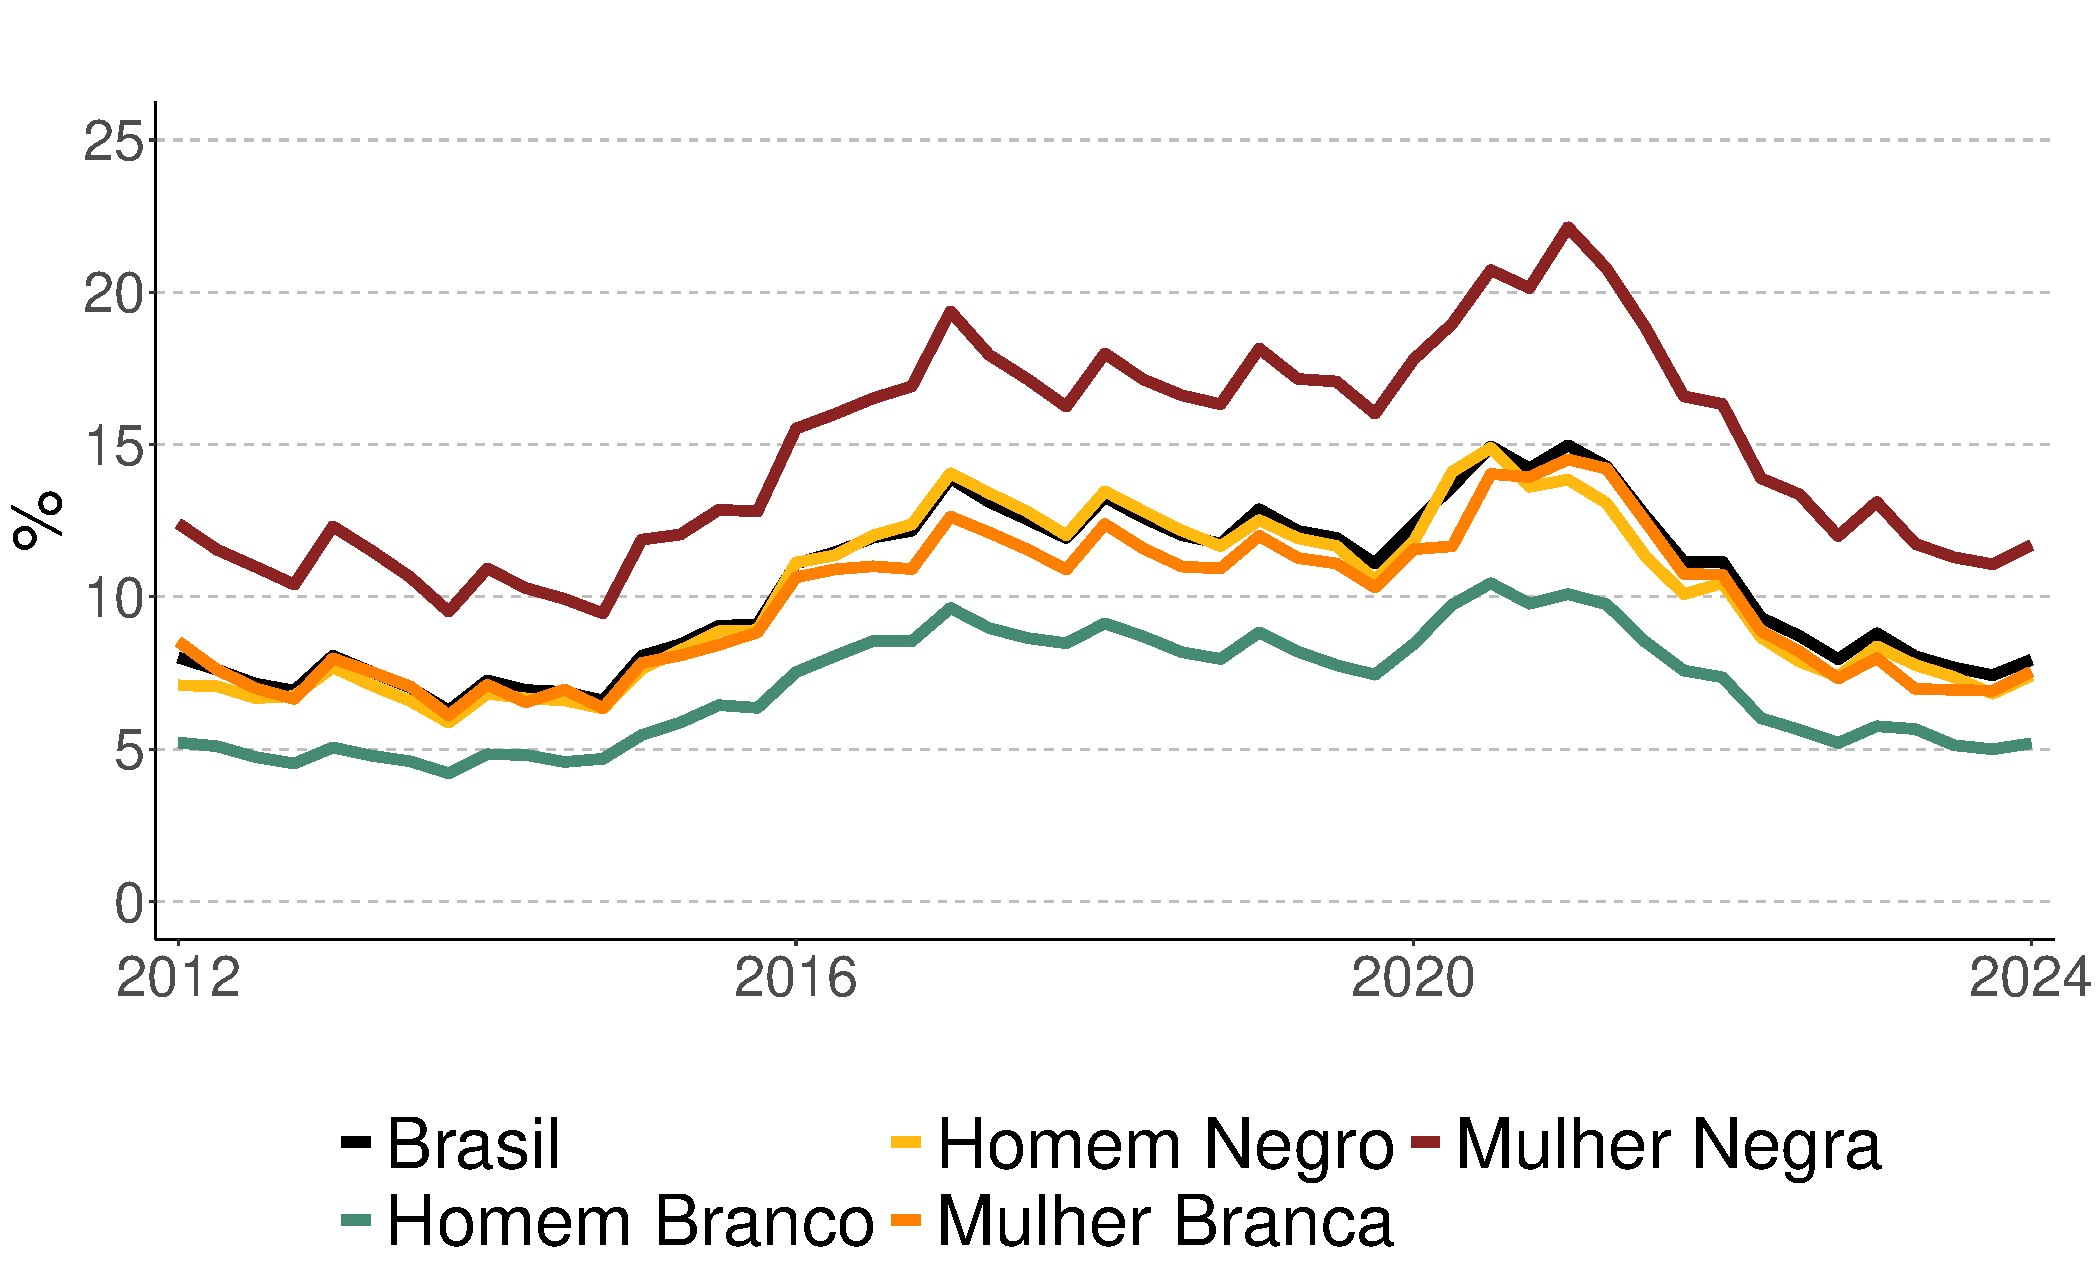
\includegraphics[width = 0.75\textwidth]{../figures_output/pea_br_gen_raca.pdf}
		\end{figure}
	\end{frame}			
	
	
	\begin{frame}{Taxa de Desemprego}
		\begin{figure}
			\centering
			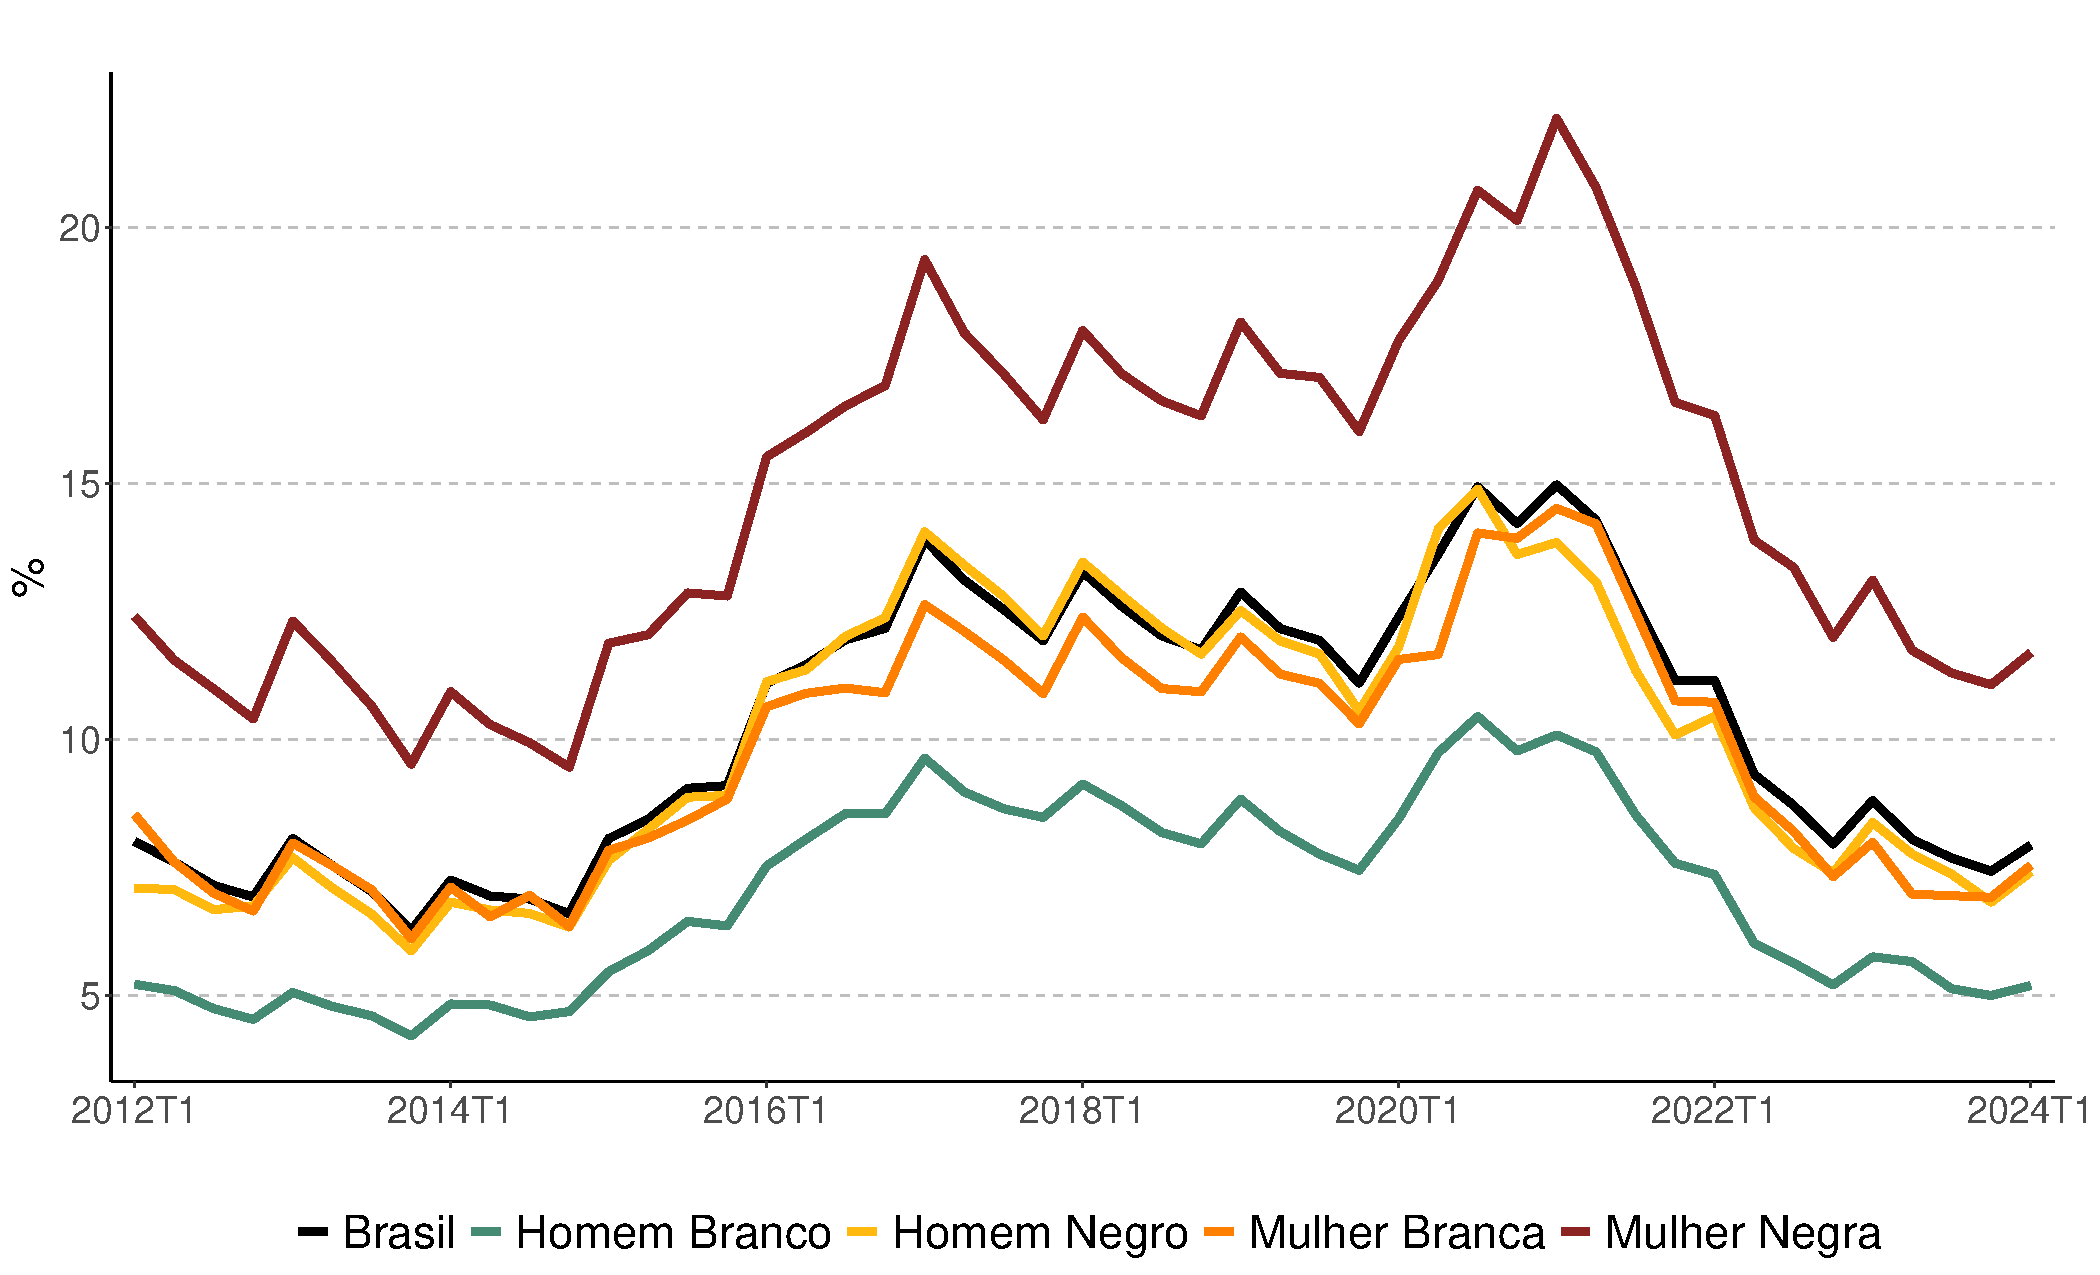
\includegraphics[width = 0.75\textwidth]{../figures_output/unemp_br_gen_raca.pdf}
		\end{figure}
	\end{frame}			
	
	
	\begin{frame}{Rendimento Habitual Real Médio de Todos os Trabalhos}
		\begin{figure}
			\centering
			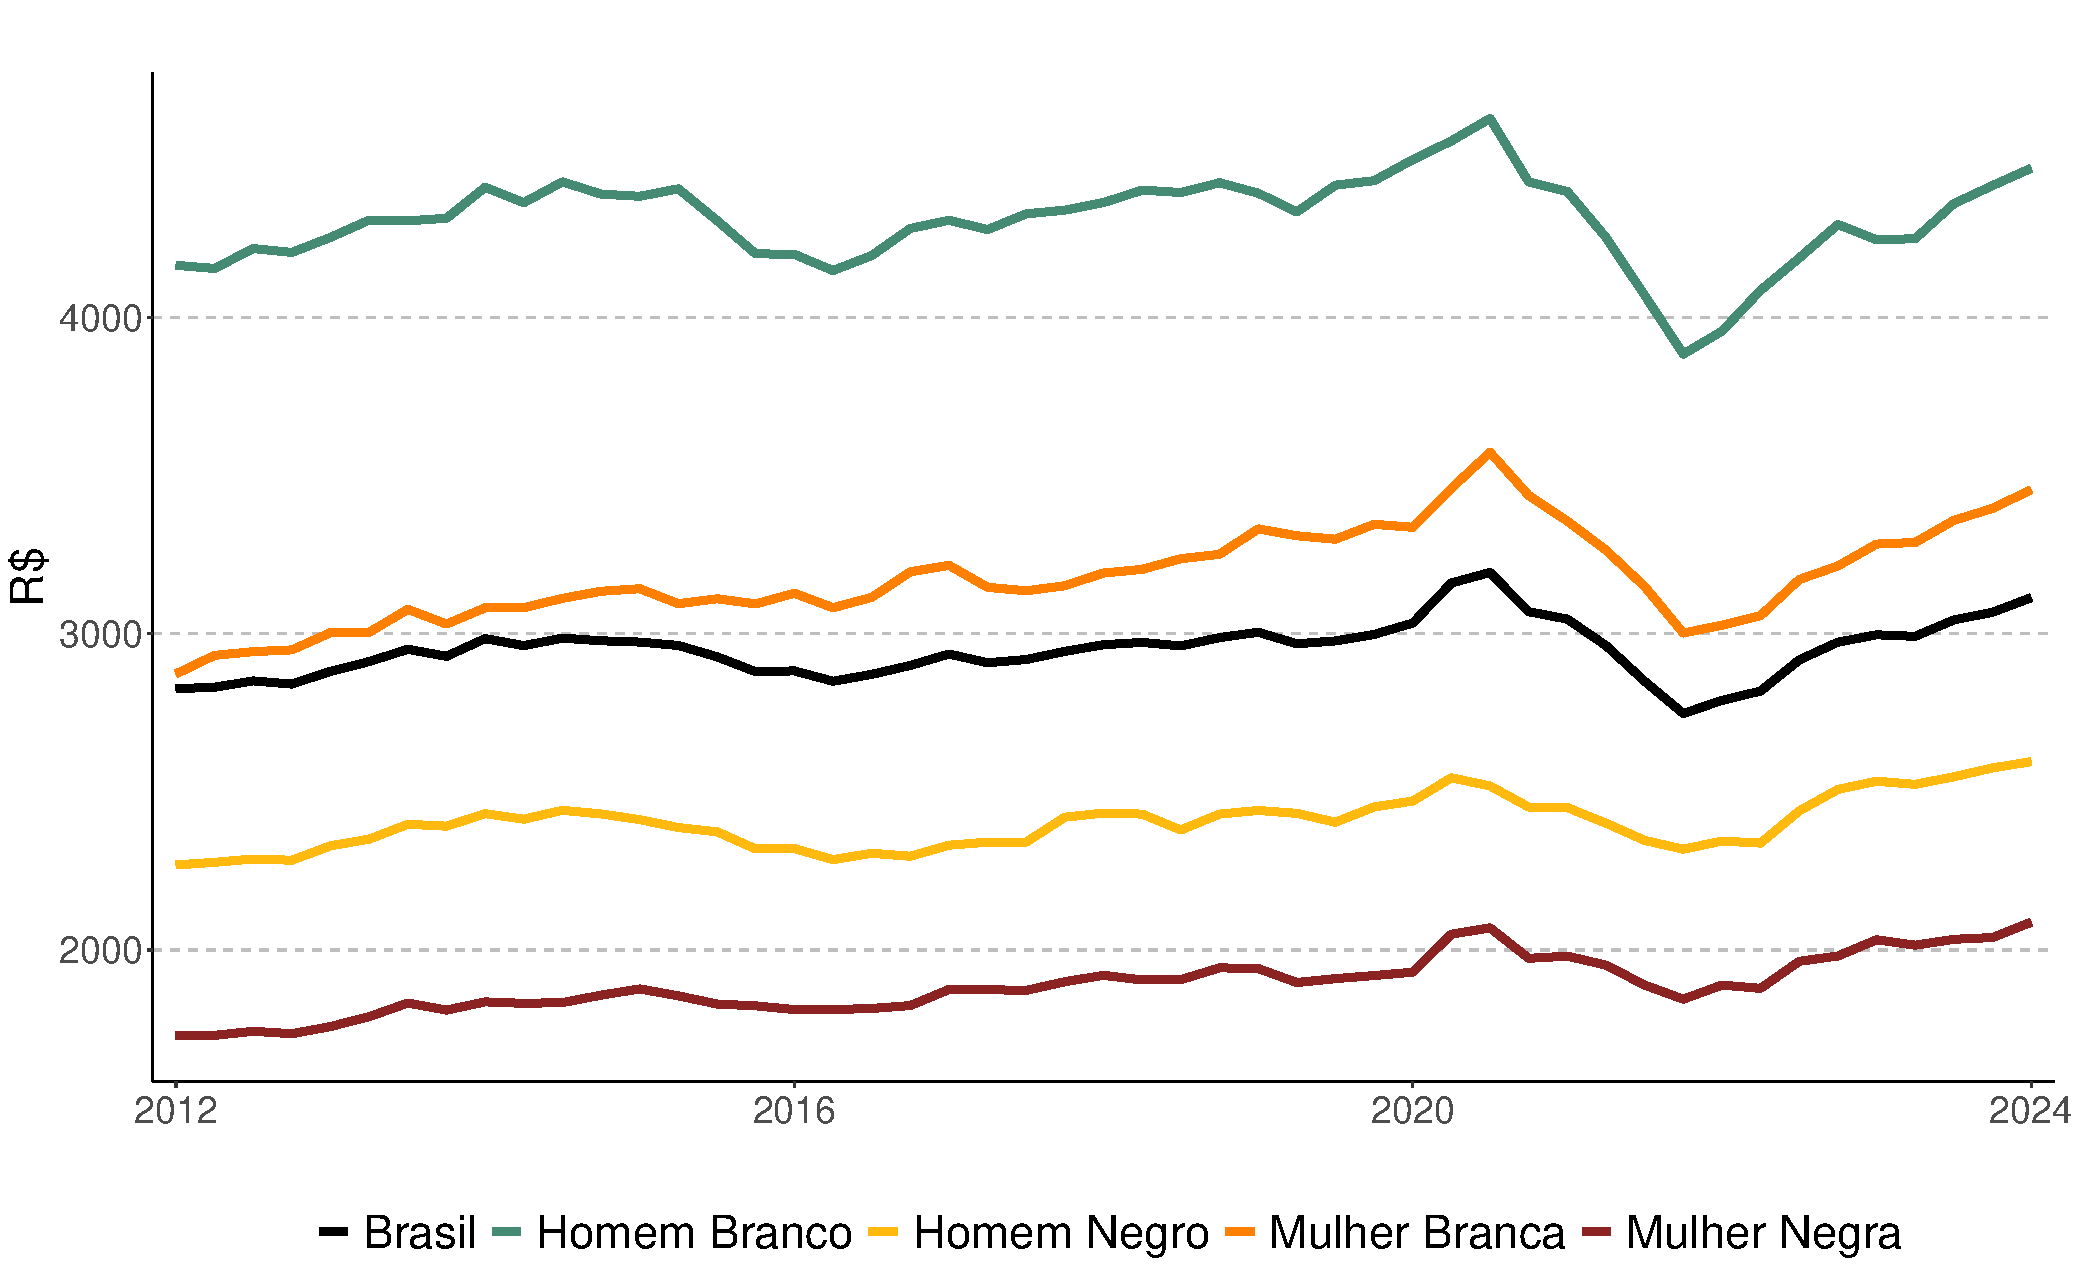
\includegraphics[width = 0.75\textwidth]{../figures_output/rendimento_habitual_br_gen_raca.pdf}
		\end{figure}
	\end{frame}
	
	
	\begin{frame}{Massa Salarial de Todos os Rendimentos Habituais do Trabalho}
		\begin{figure}
			\centering
			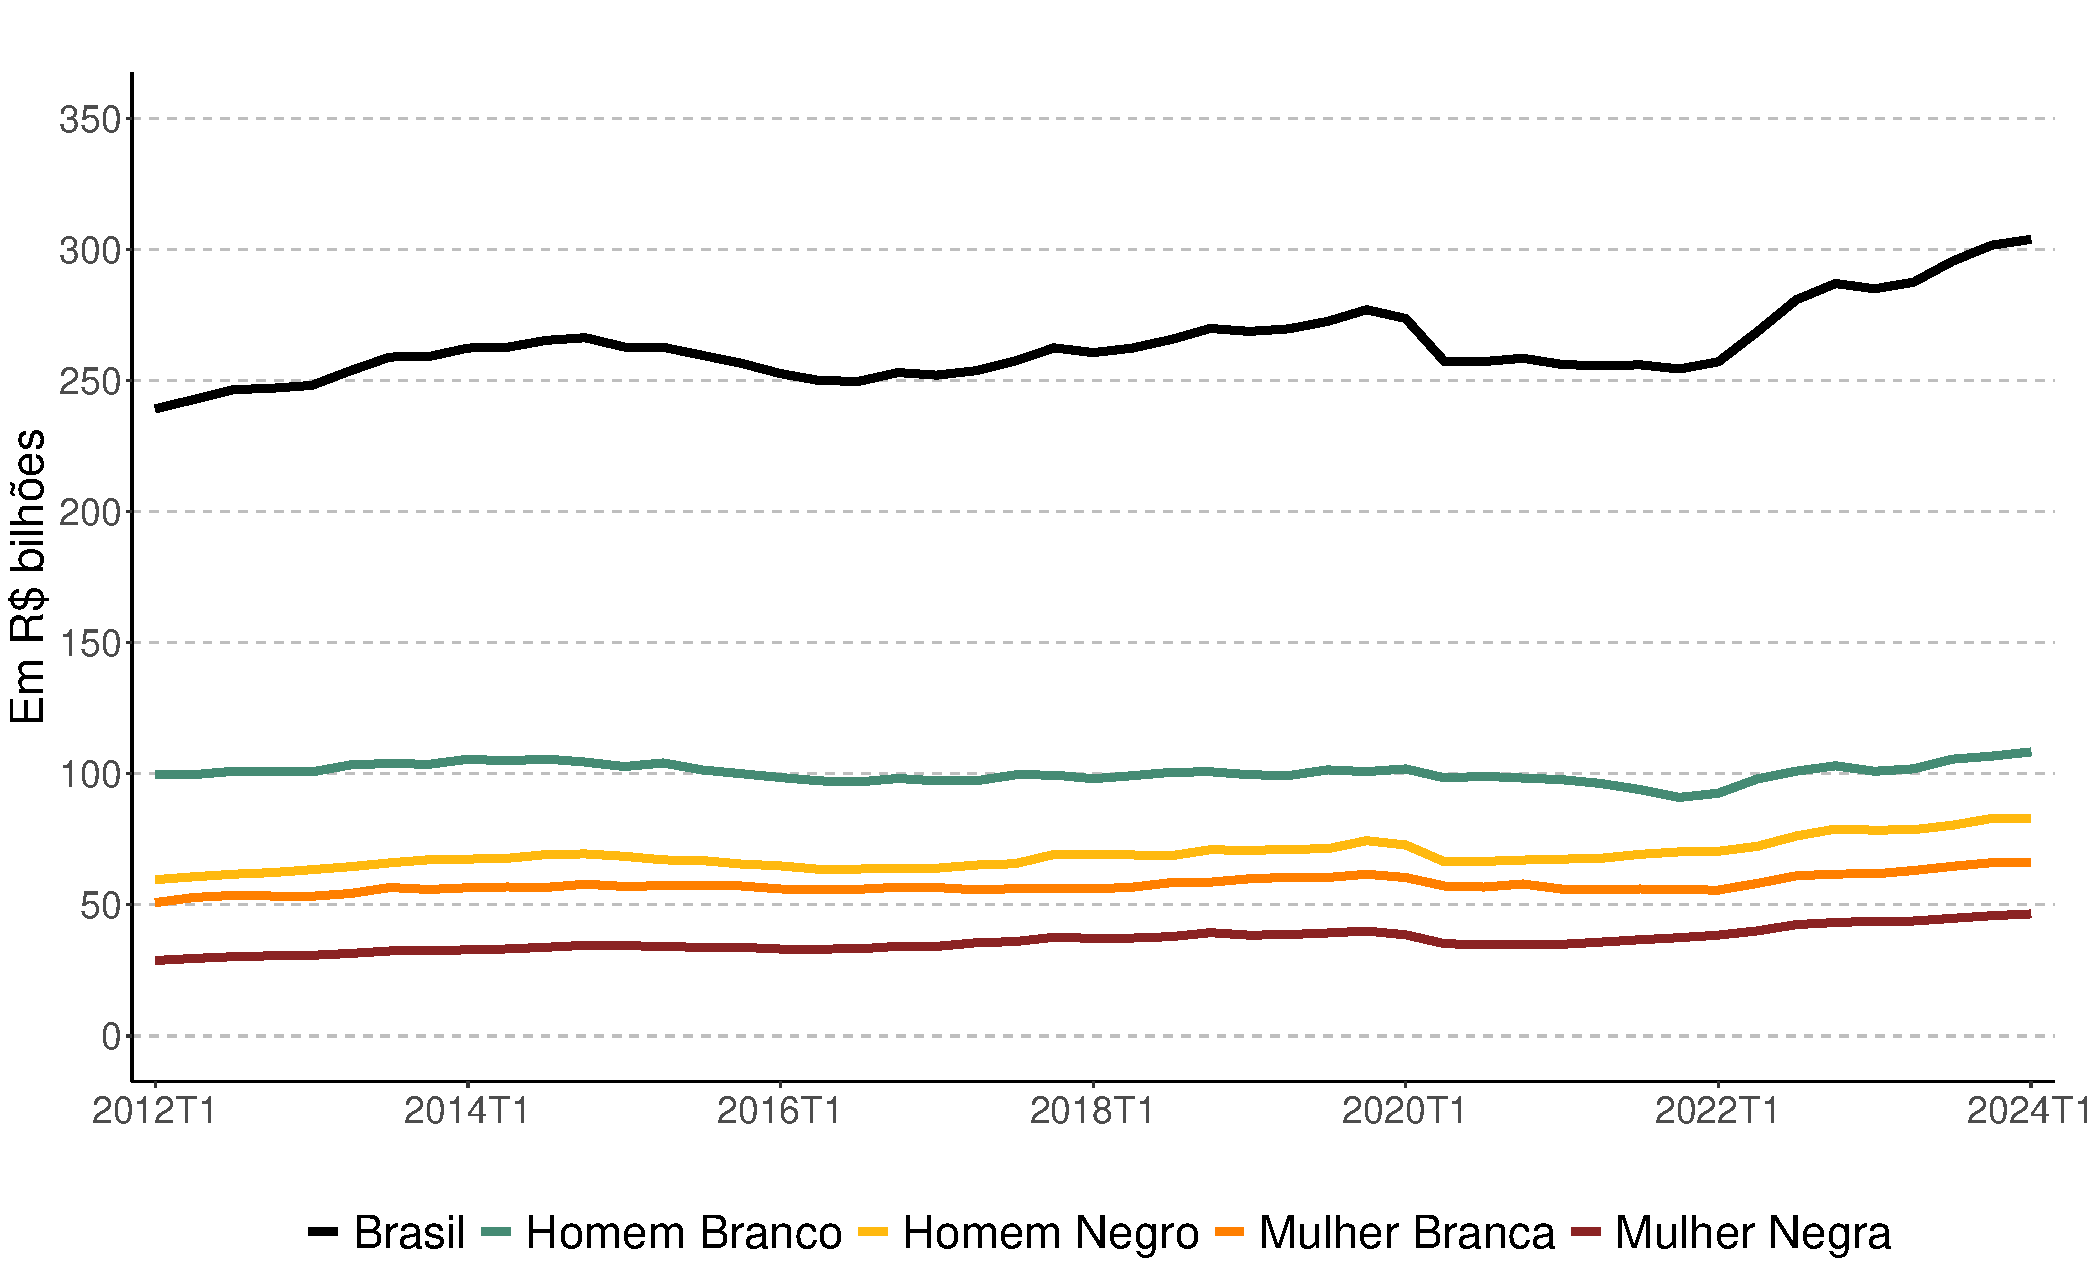
\includegraphics[width = 0.75\textwidth]{../figures_output/massa_habitual_br_gen_raca.pdf}
		\end{figure}
	\end{frame}
	
	
	\begin{frame}{Gini}
		\begin{figure}
			\centering
			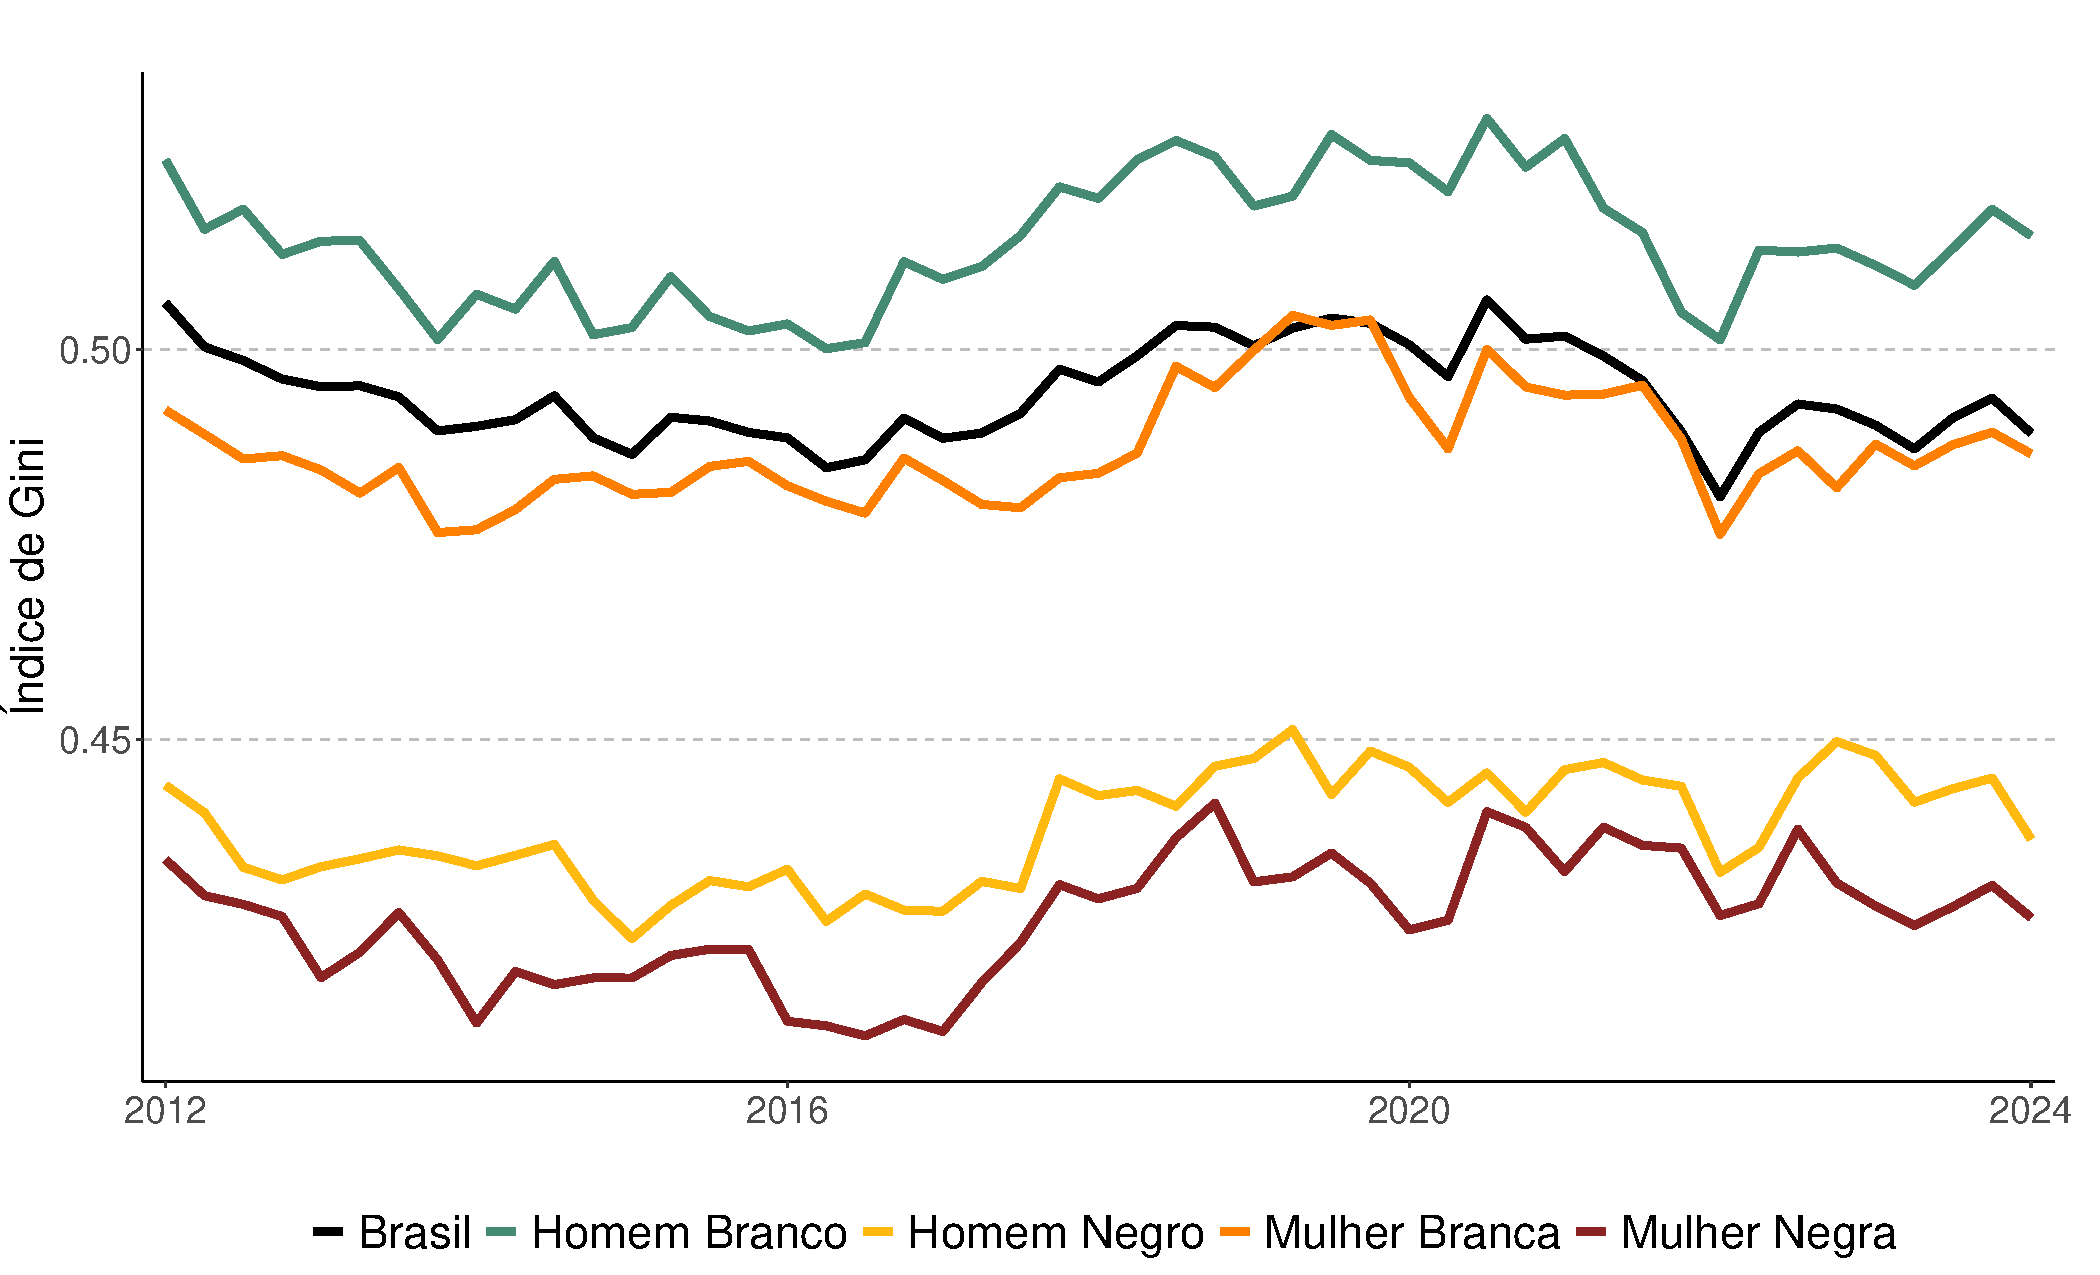
\includegraphics[width = 0.75\textwidth]{../figures_output/gini_br_gen_raca.pdf}
		\end{figure}
	\end{frame}
	
	\section{O Mercado de Trabalho Recente}
	\begin{frame}{População Economicamente Ativa}
		\begin{figure}
			\centering
			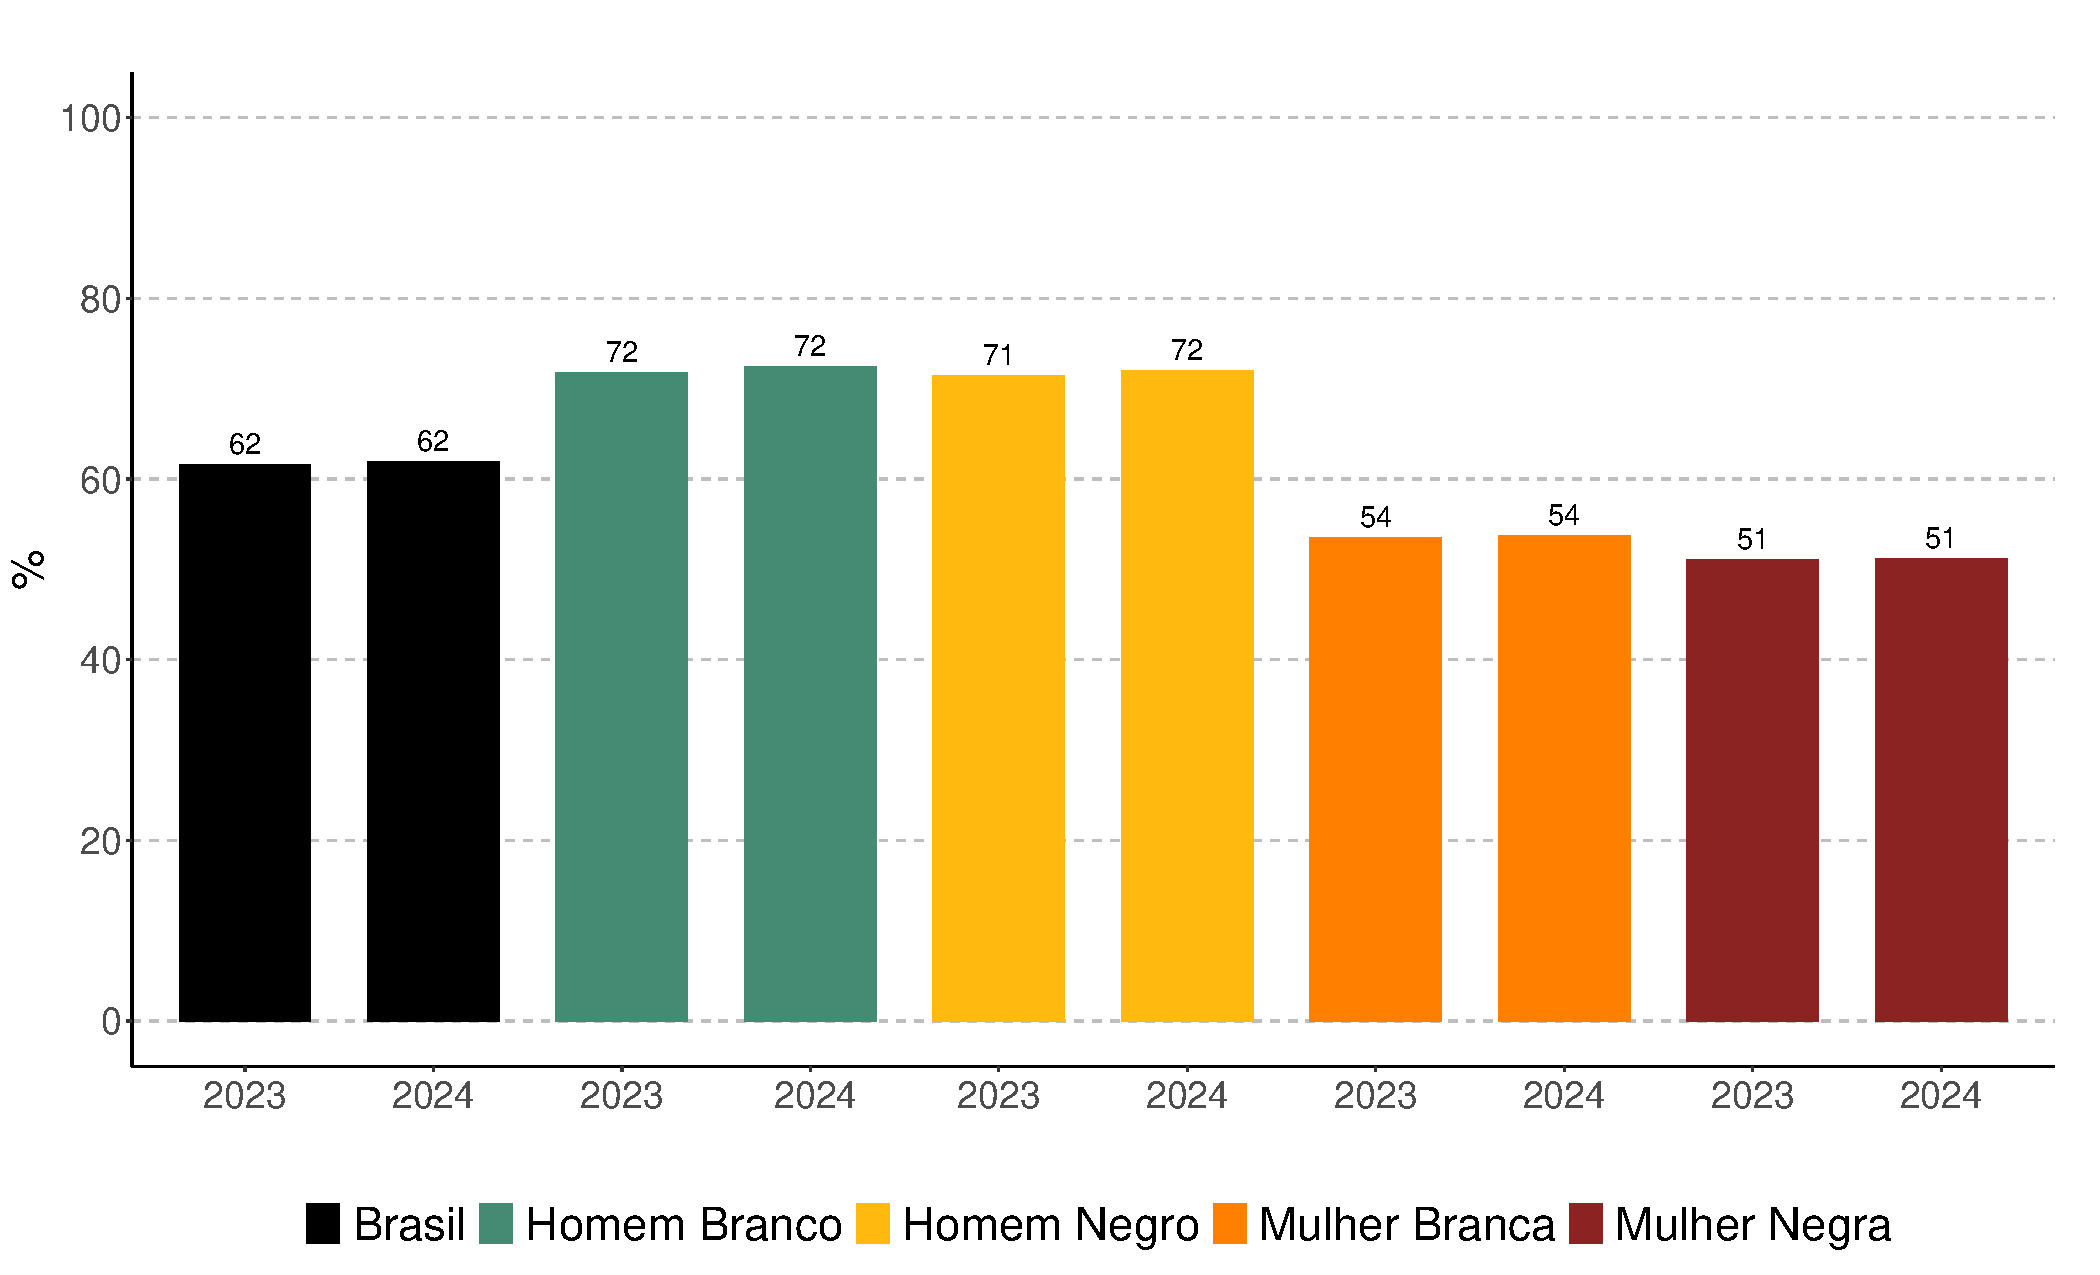
\includegraphics[width = 0.75\textwidth]{../figures_output/pea.pdf}
		\end{figure}
	\end{frame}			
	
	\begin{frame}{Taxa de Desemprego}
		\begin{figure}
			\centering
			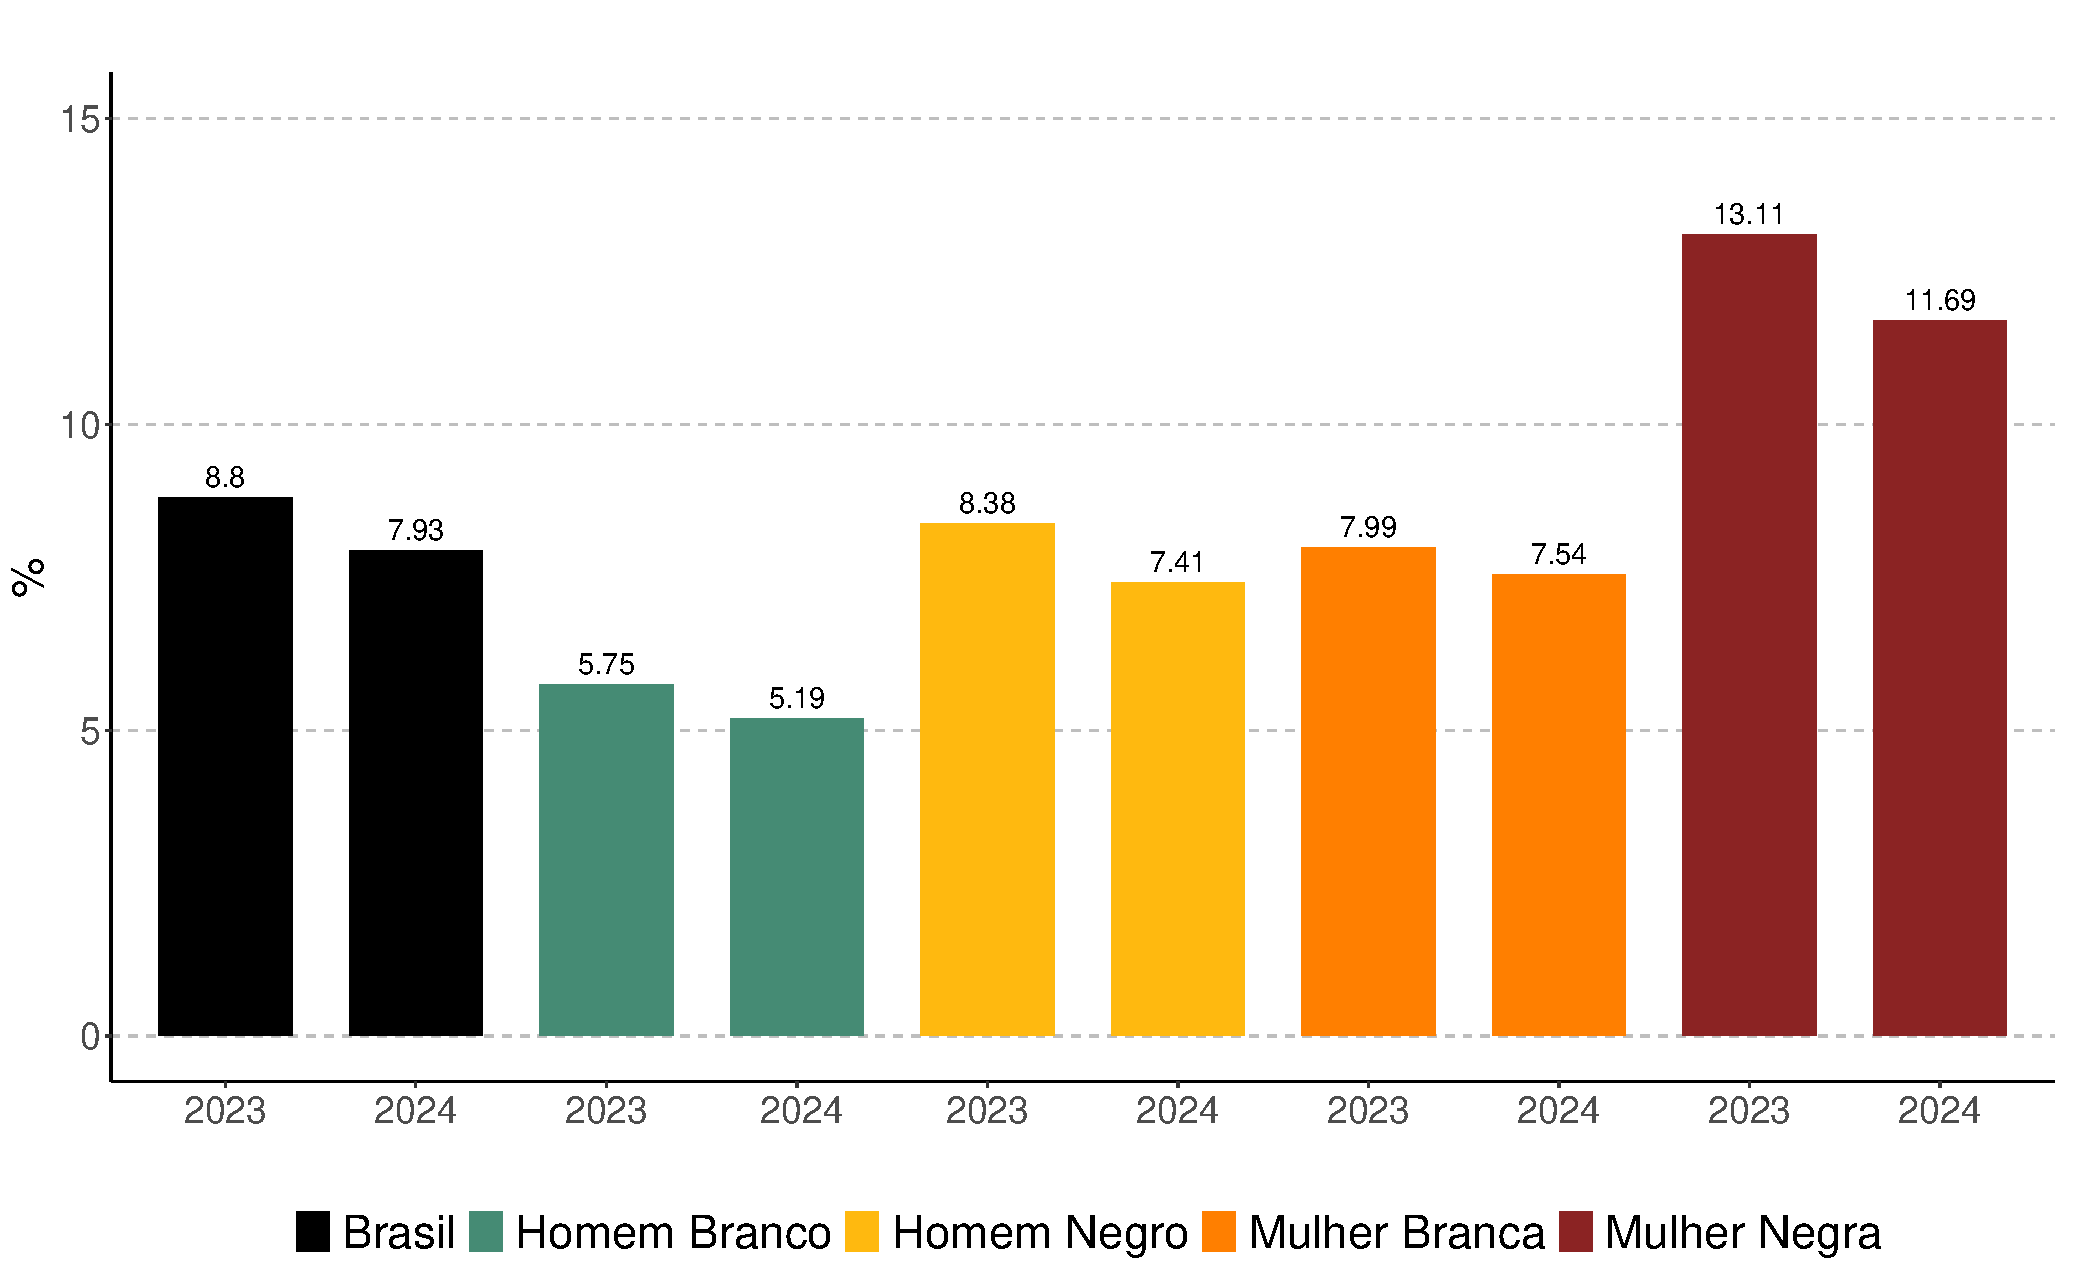
\includegraphics[width = 0.75\textwidth]{../figures_output/unemp.pdf}
		\end{figure}
	\end{frame}	
	
	\begin{frame}{Massa Salarial Habitual}
		\begin{figure}
			\centering
			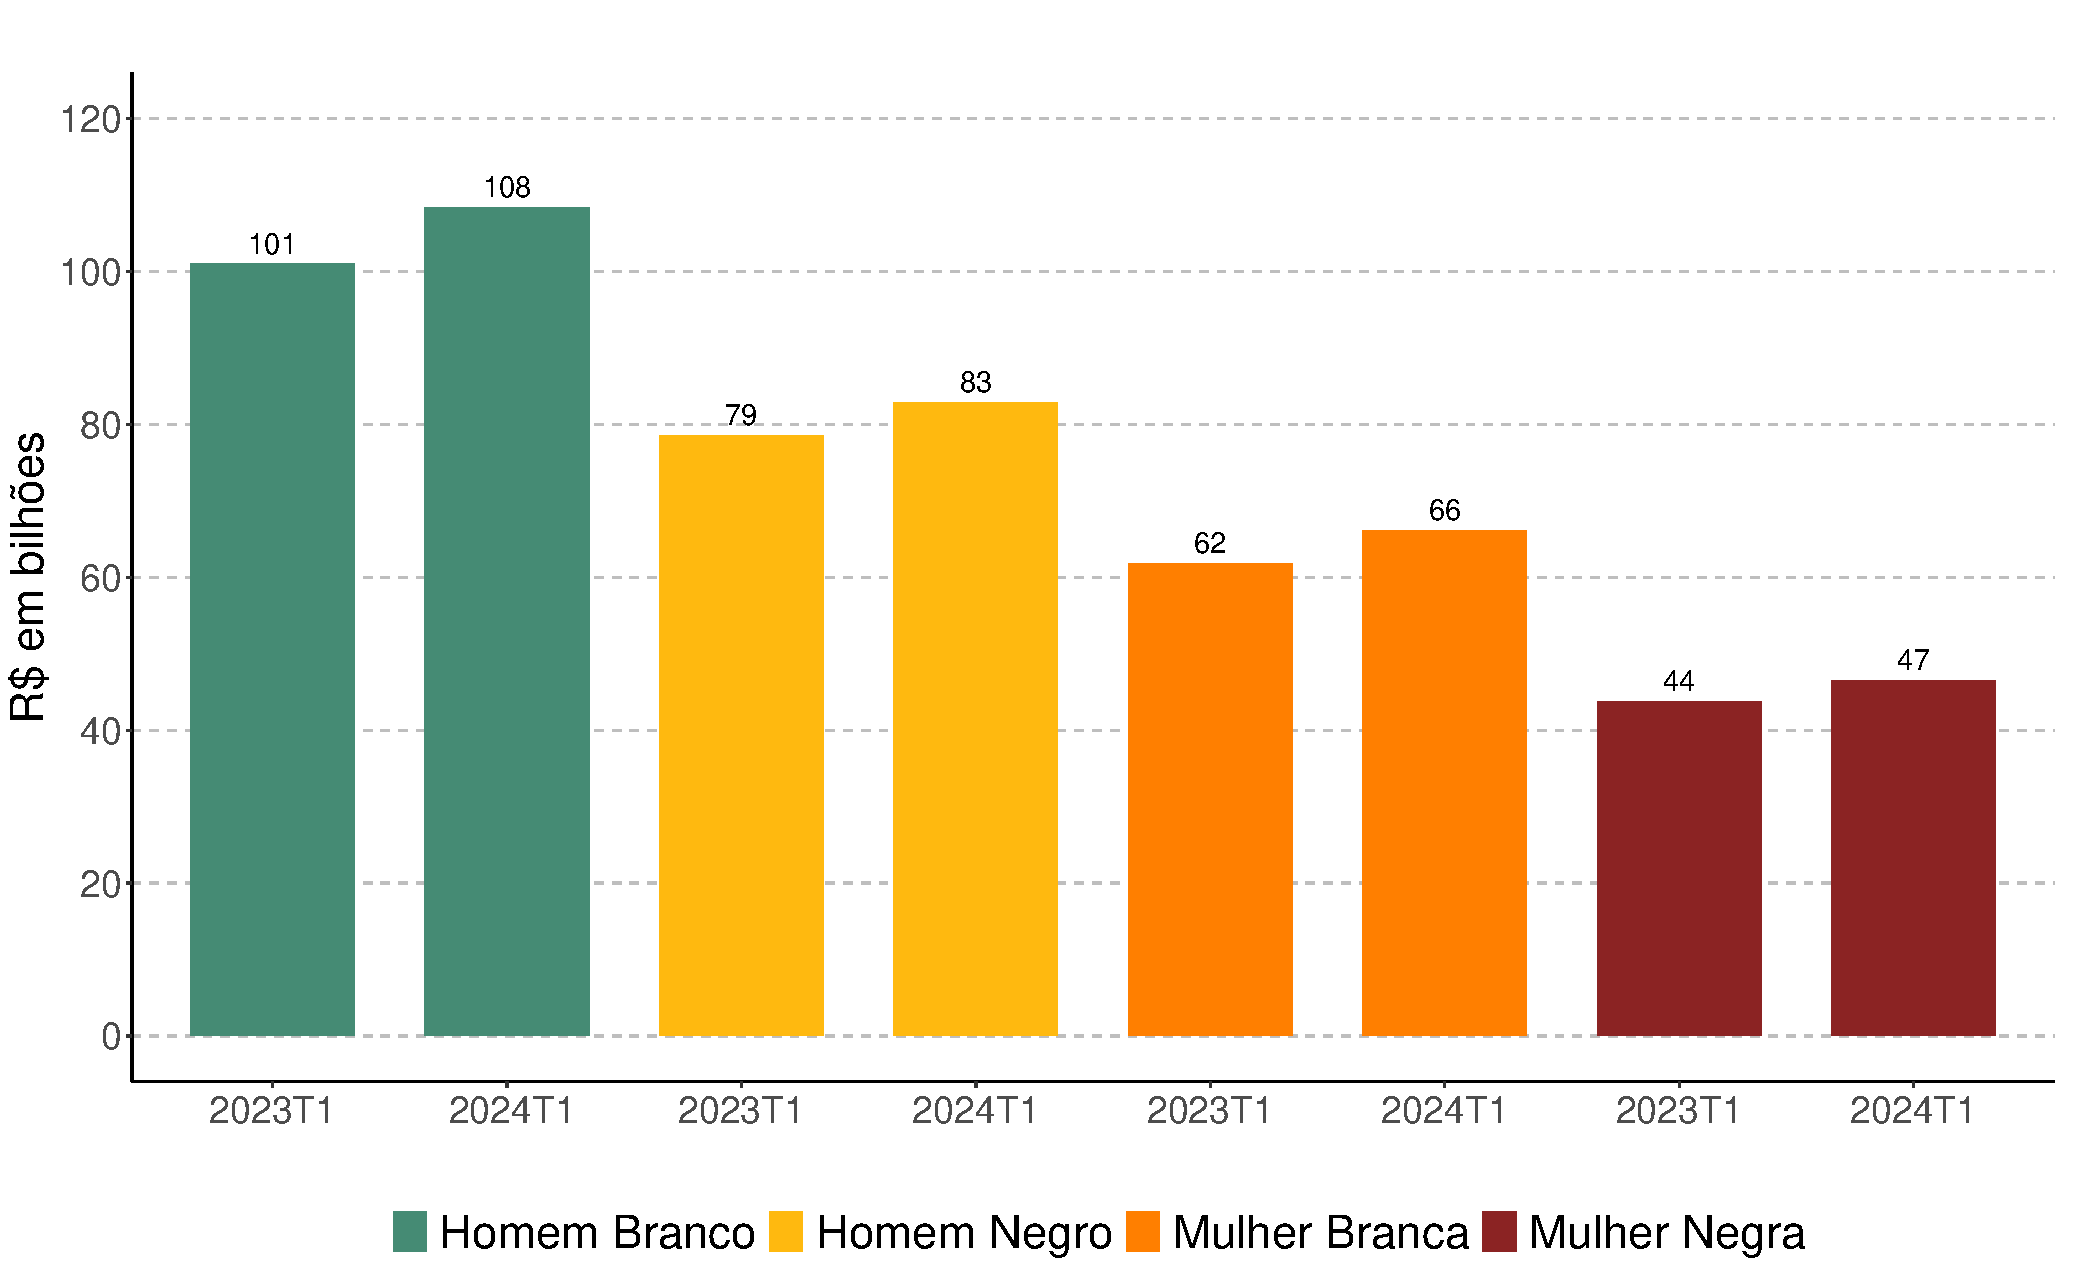
\includegraphics[width = 0.75\textwidth]{../figures_output/massa_habitual.pdf}
		\end{figure}
	\end{frame}
	
	
	\section{Os Grupos Minoritários em Relação ao Homem Branco} 
	\begin{frame}{Fração da PEA em Relação ao Homem Branco}
		\begin{figure}
			\centering
			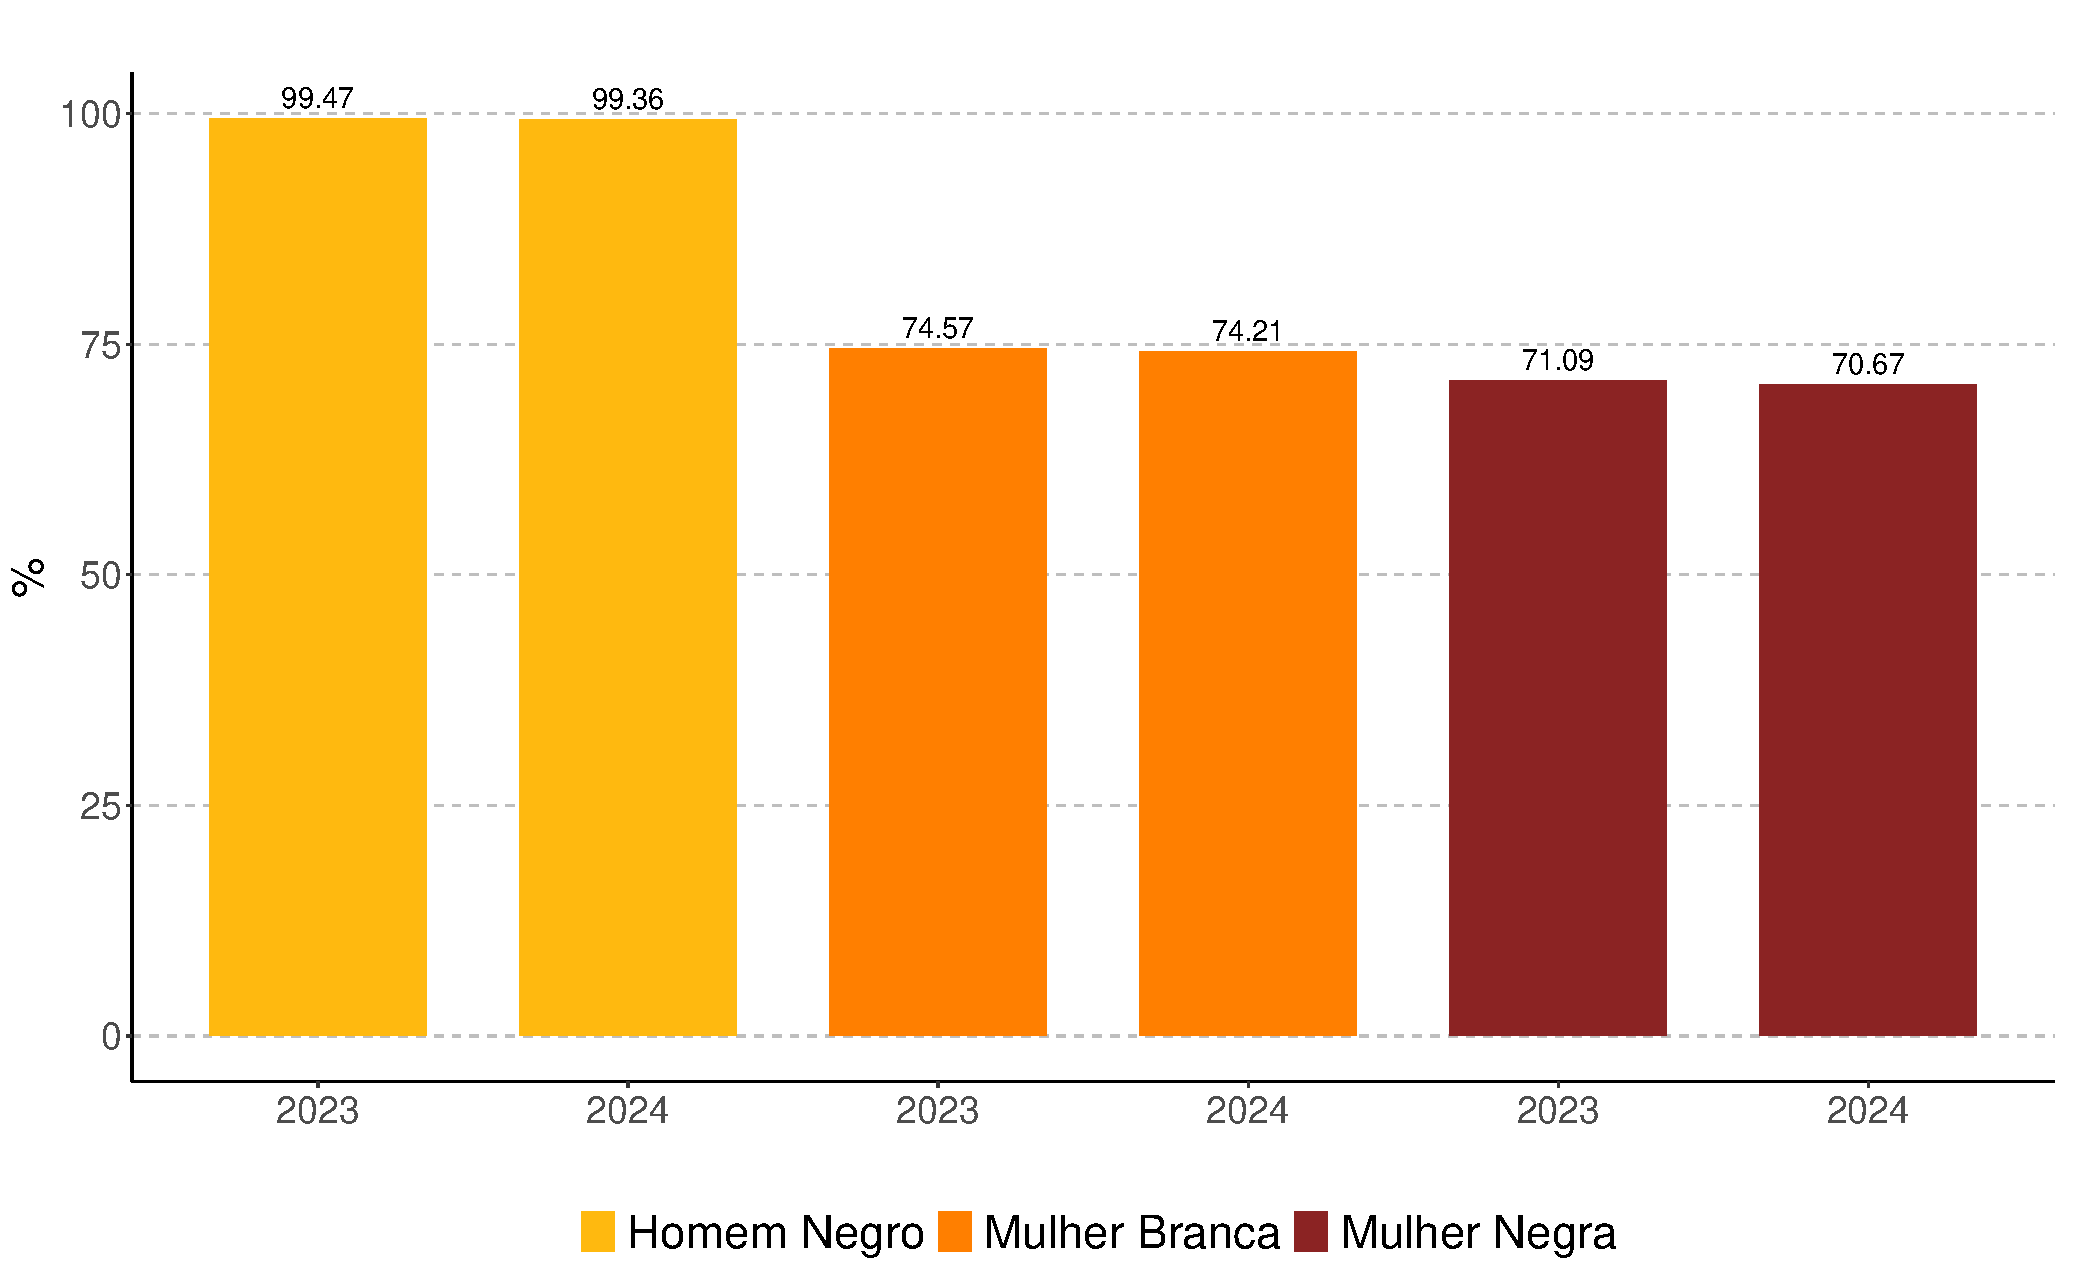
\includegraphics[width = 0.75\textwidth]{../figures_output/frac_pea.pdf}
		\end{figure}
	\end{frame}
	
	\begin{frame}{Razão de Chances de Estar Desempregado em Relação ao Homem Branco}
		\begin{figure}
			\centering
			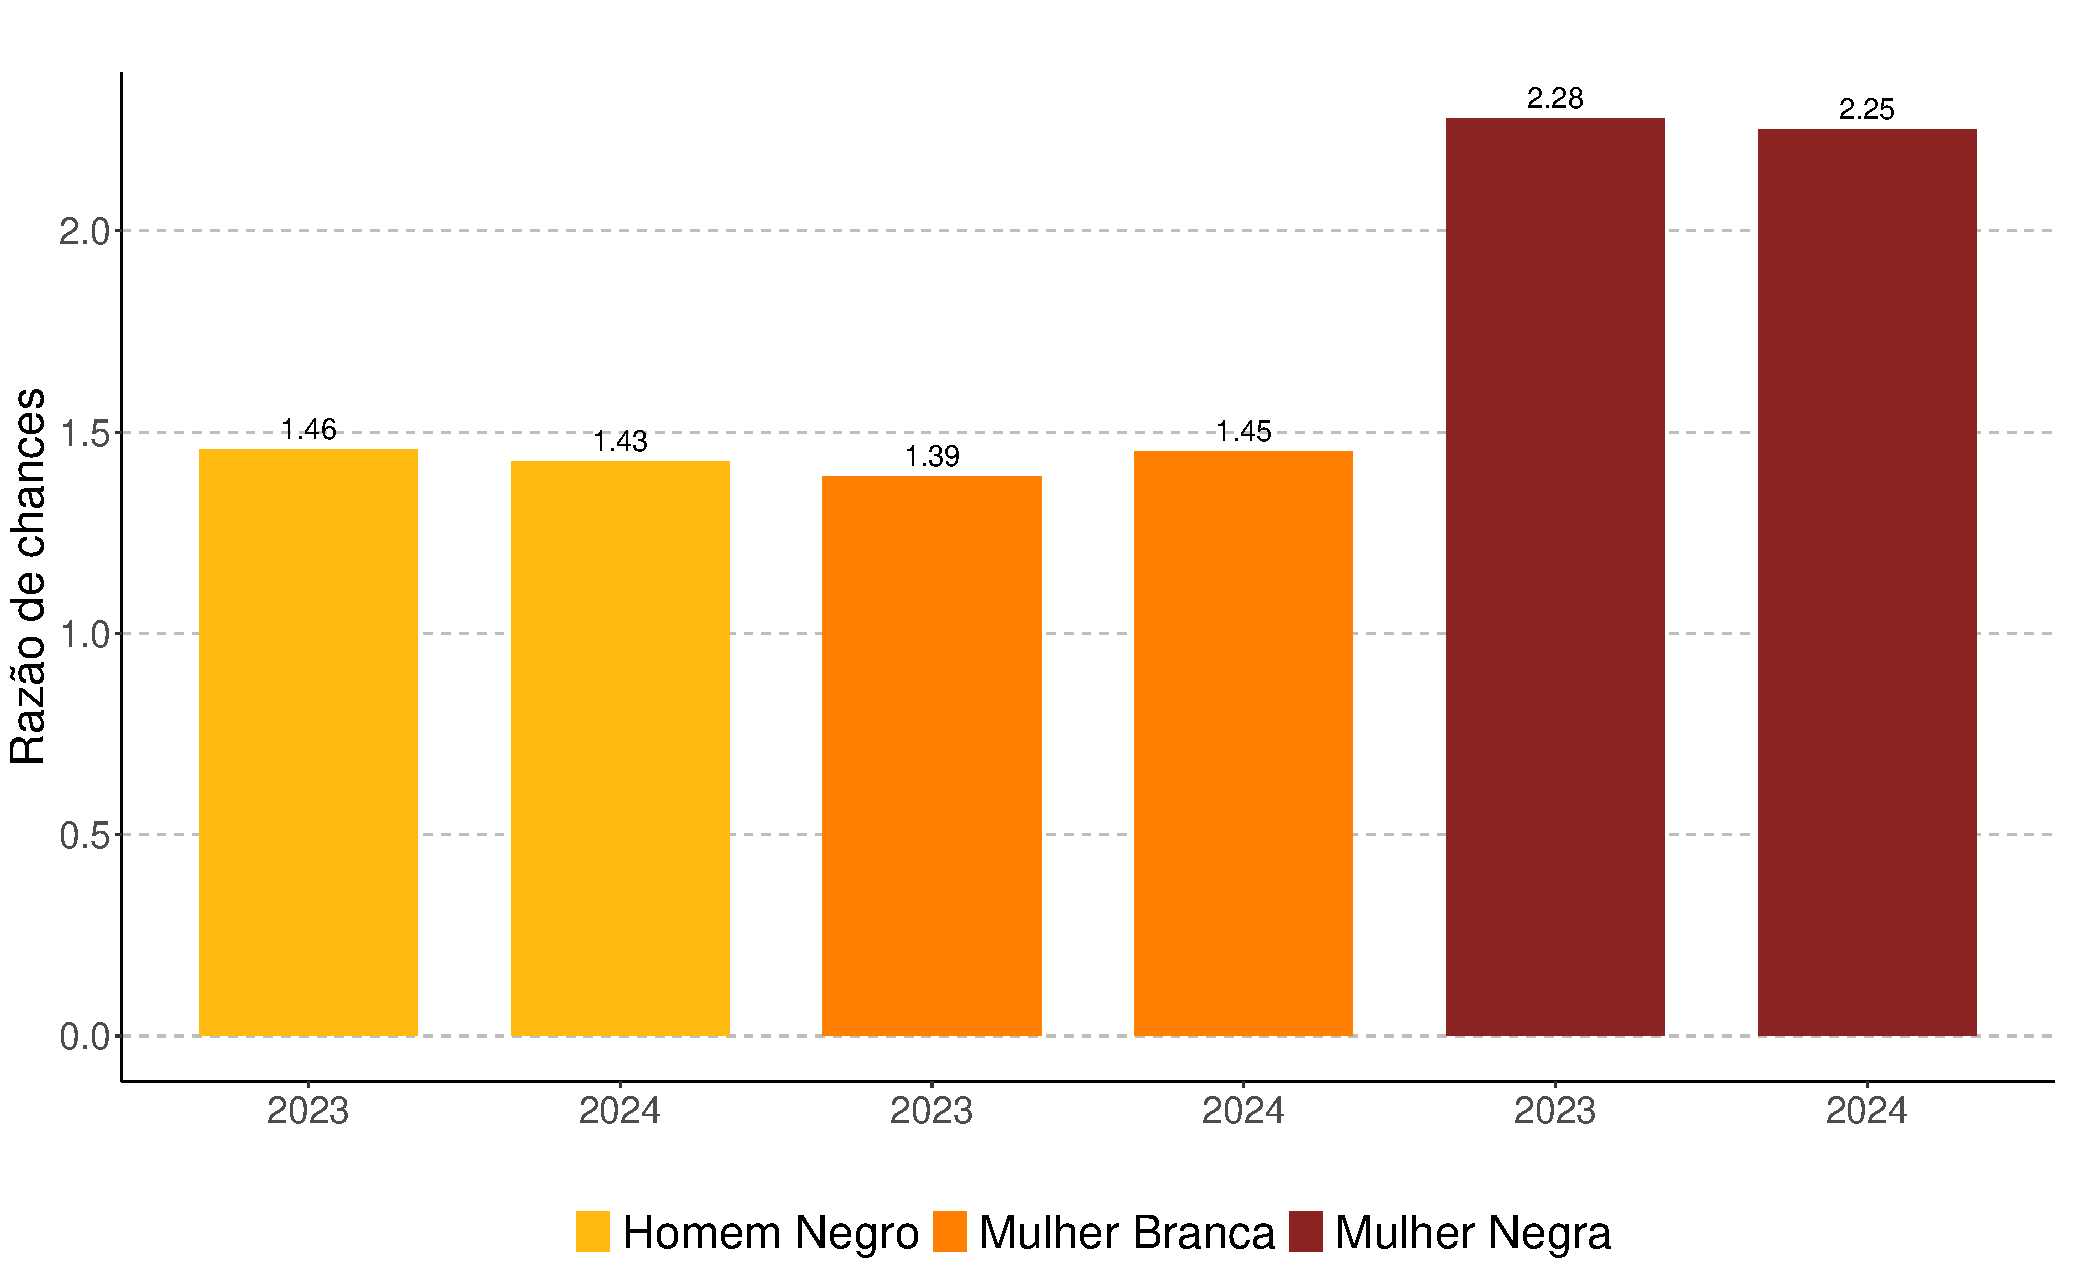
\includegraphics[width = 0.75\textwidth]{../figures_output/frac_unemp.pdf}
		\end{figure}
	\end{frame}
	
	\begin{frame}{Proporção do Rendimento Habitual em Relação ao Homem Branco}
		\begin{figure}
			\centering
			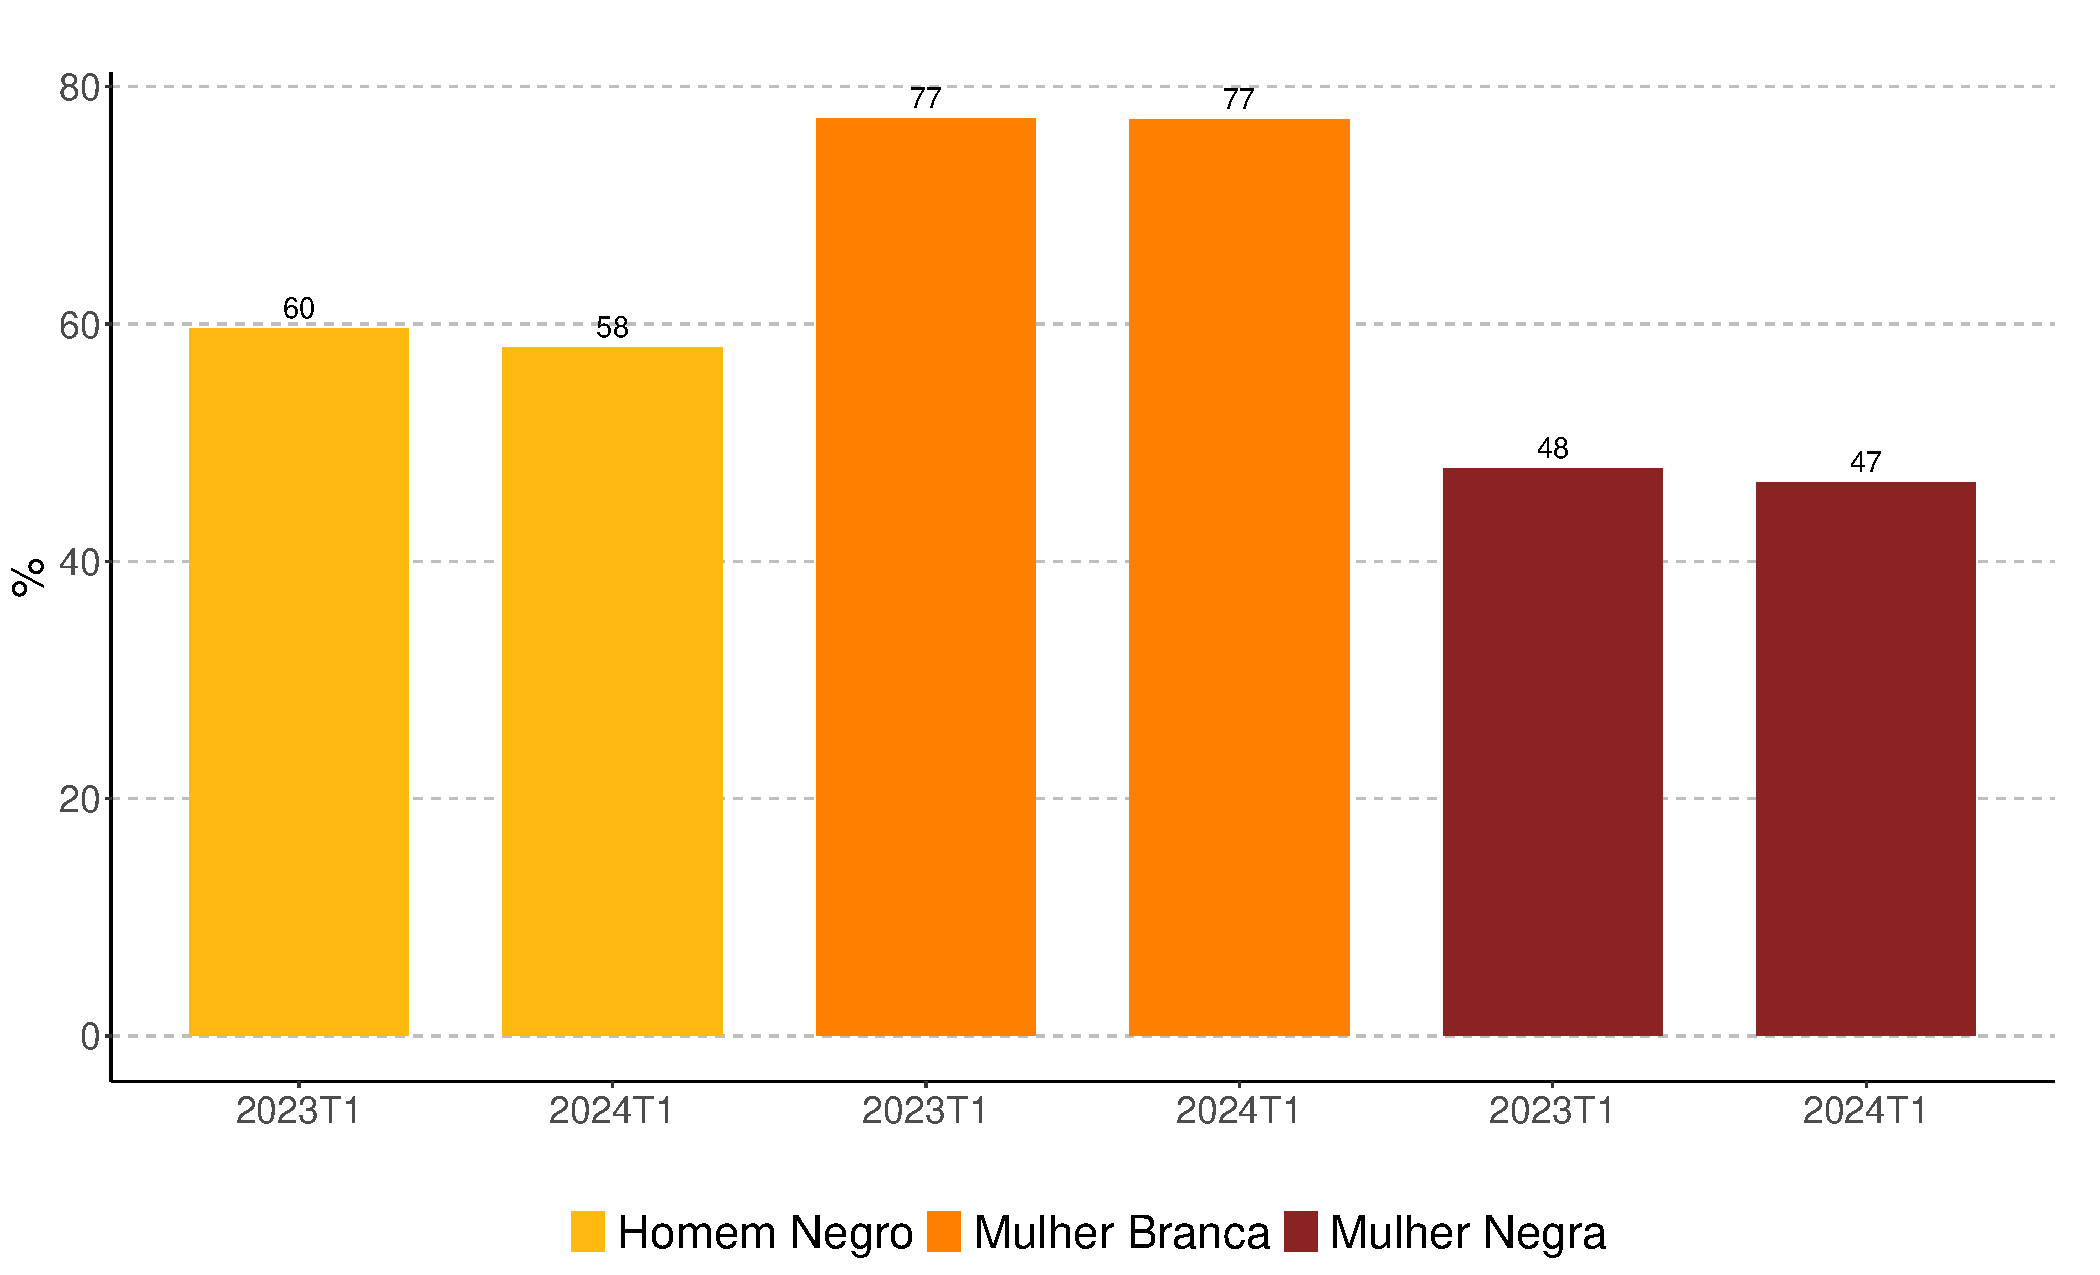
\includegraphics[width = 0.75\textwidth]{../figures_output/frac_rendimento_habitual.pdf}
		\end{figure}
	\end{frame}

	\begin{frame}{Proporção da Massa Habitual em Relação ao Homem Branco}
		\begin{figure}
			\centering
			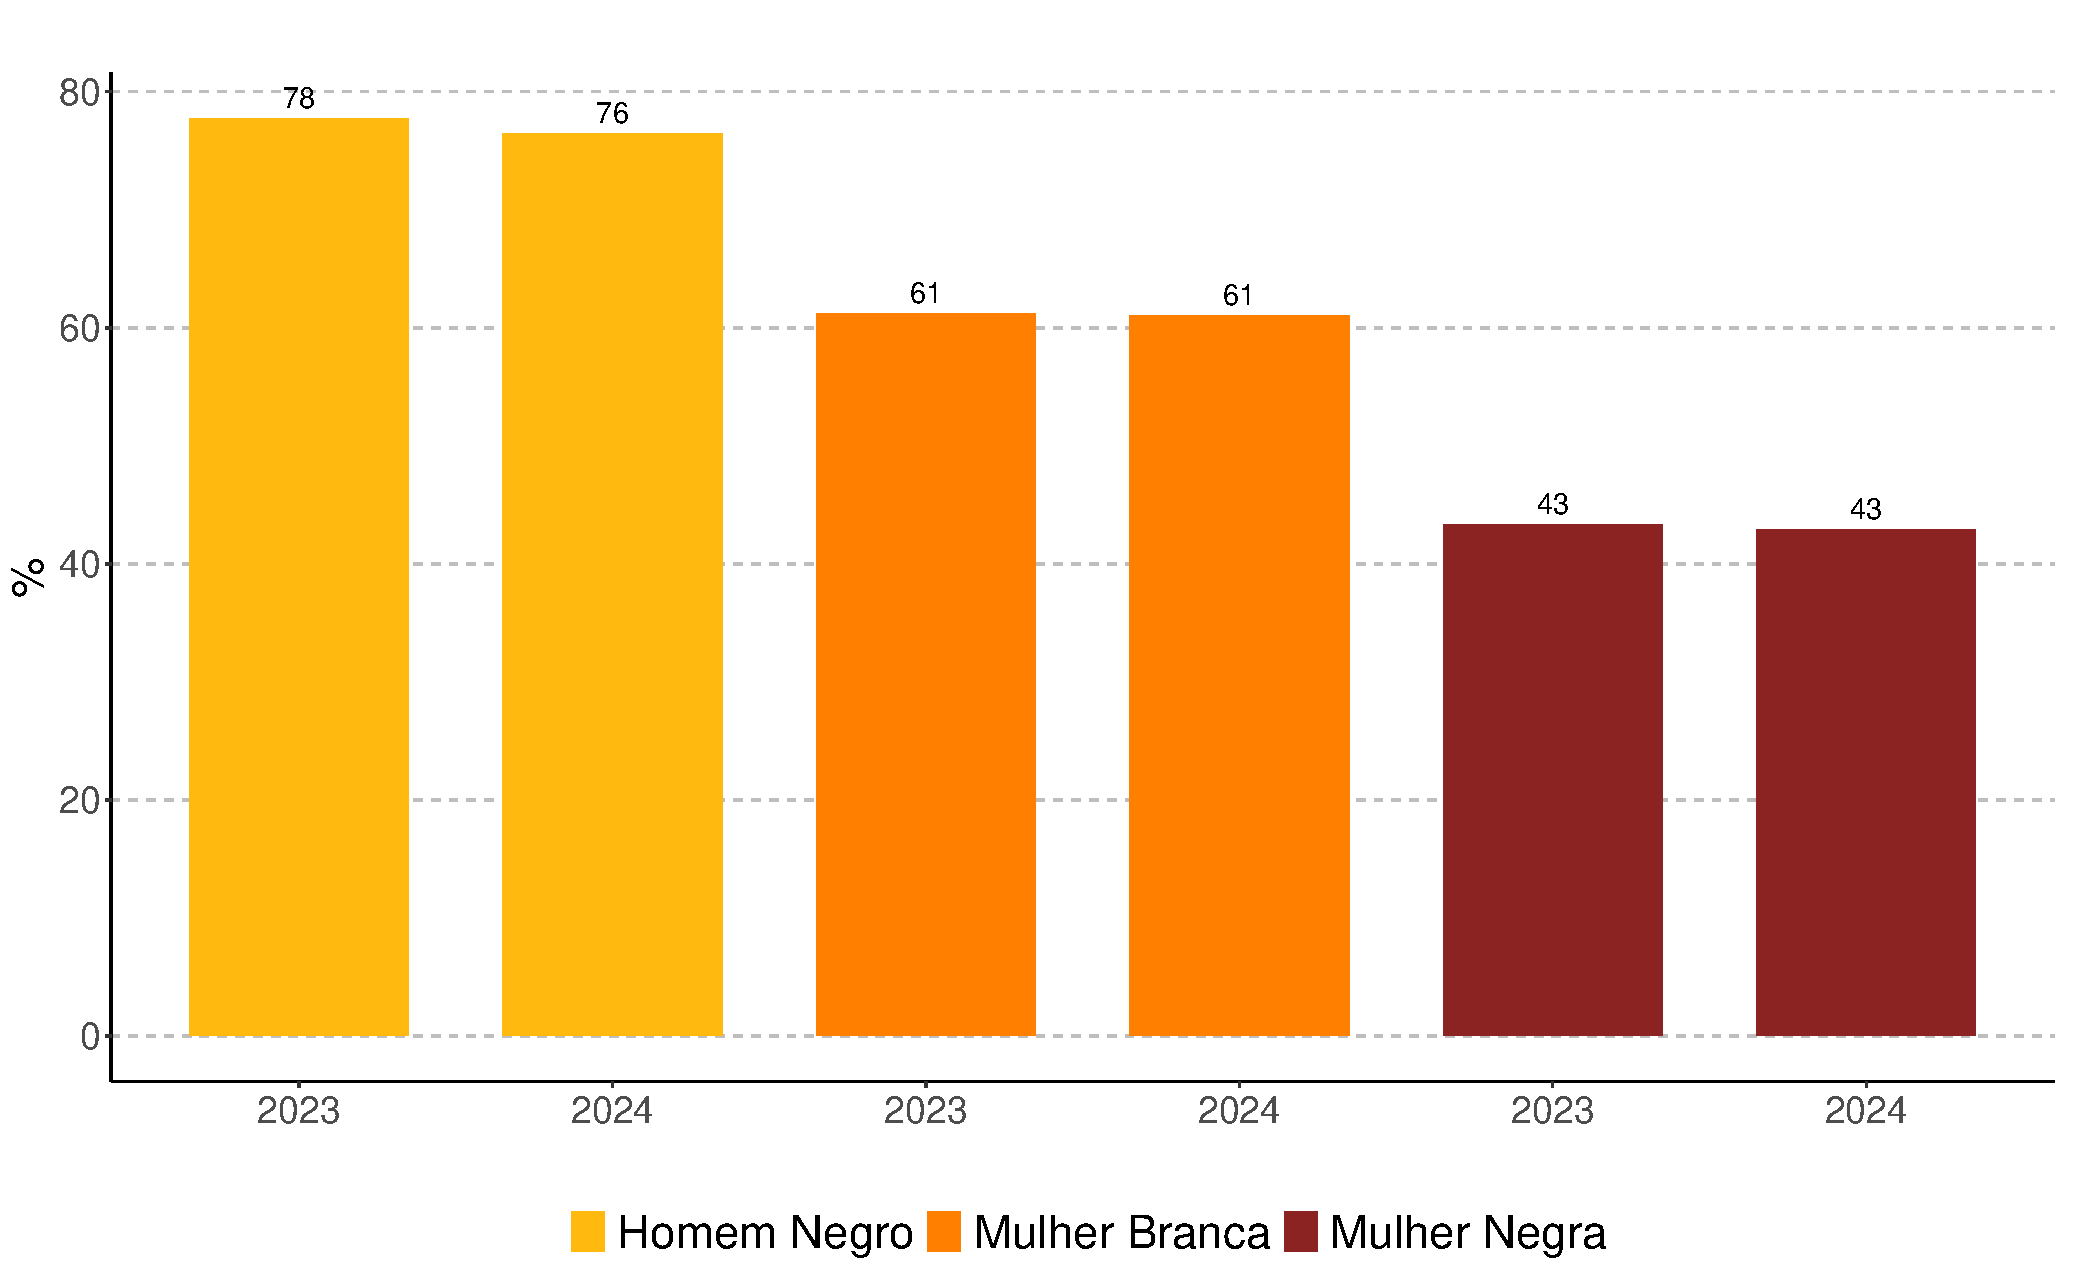
\includegraphics[width = 0.75\textwidth]{../figures_output/frac_massa_habitual.pdf}
		\end{figure}
	\end{frame}
	
	
	\begin{frame}{Razão de Chances Gini em Relação ao Homem Branco}
		\begin{figure}
			\centering
			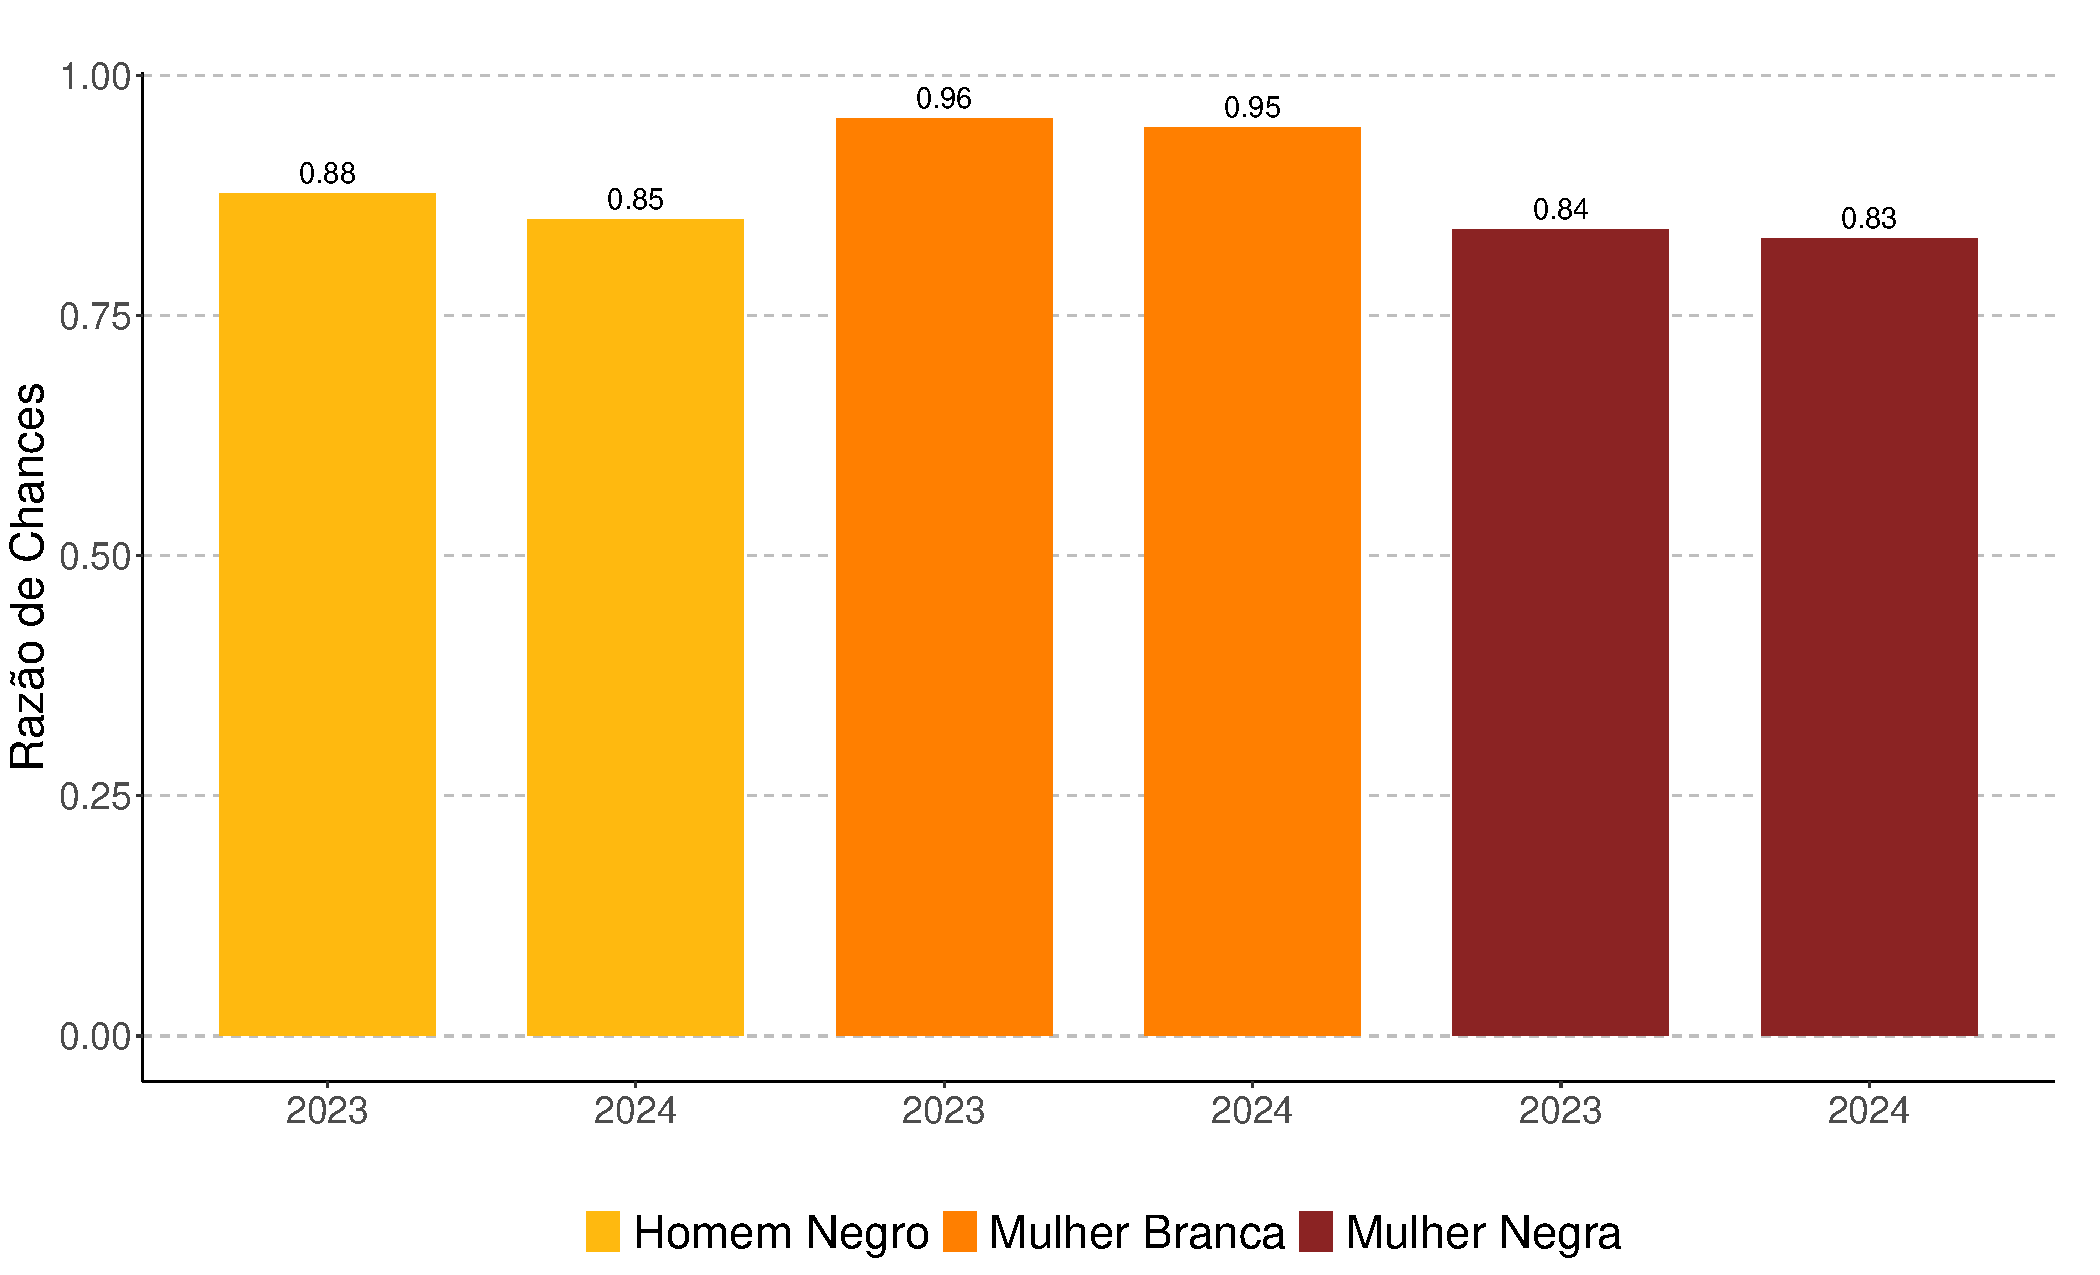
\includegraphics[width = 0.75\textwidth]{../figures_output/frac_gini.pdf}
		\end{figure}
	\end{frame}
	
	\section{Composição da Base e do Topo}
	\begin{frame}{A Base e o Topo da Distribuição}
		\begin{figure}
			\centering
			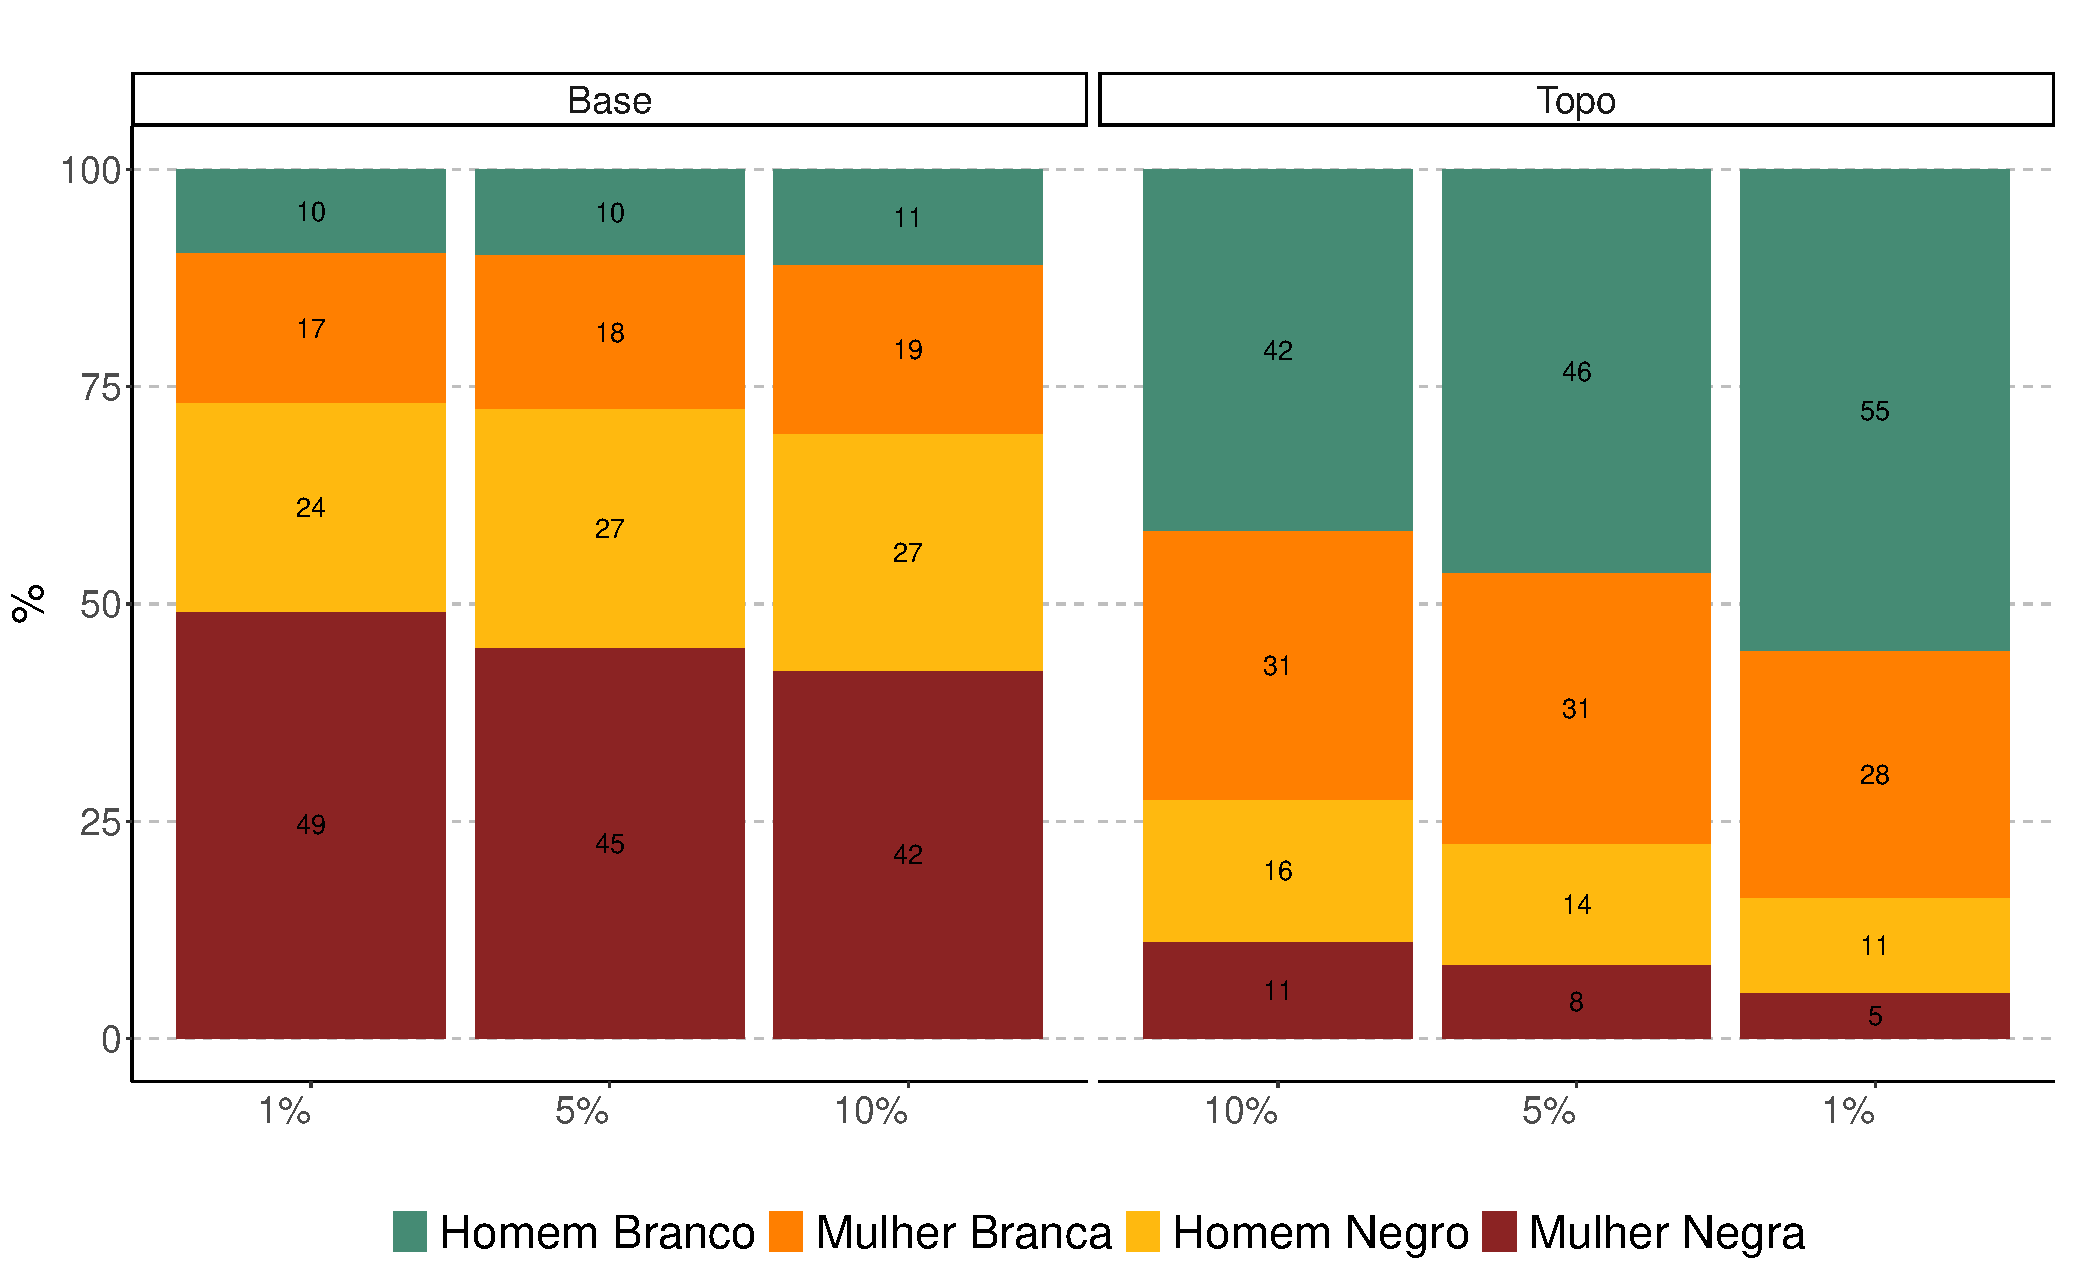
\includegraphics[width = 0.75\textwidth]{../figures_output/top_bottom.pdf}
		\end{figure}
	\end{frame}
	
\section{A Discriminação no Mercado de Trabalho}

\begin{frame}{Salário}
	Função salarial:
	\begin{equation}
		\log(y_{iR}) = \alpha + X_{i}\beta + \gamma R_{i} + \epsilon_{i}
	\end{equation}
	
	Salário esperado para brancos:
	\begin{equation}
		E(y_{i}|R=0) = \alpha + E(X|R=0)\beta
	\end{equation}
	
	Salário esperado para negros:
	\begin{equation}
		E(y_{i}|R=1) = \alpha + E(X|R=1)\beta + \gamma = E(y_{i}|R=0) + \Delta X\beta + \gamma
	\end{equation}
\end{frame}

\begin{frame}{Massa Salarial}
	Massa Salarial:
	\begin{equation}
		\sum y_{i} = N \sum y_{i}/N = N \bar{y}
	\end{equation}
	
	Massa entre brancos e negros:
	\begin{equation}
		\sum y_{i} = N_{0} \bar{y}_{0} + N_{1} \bar{y}_{1}
	\end{equation}
	
	Reescrevendo:
	
	\begin{equation}
		\sum y_{i} = N_{0} E(y_{i}|R=0)  + N_{1} E(y_{i}|R=0)  + \Delta X\beta + \gamma =
		N \bar{y}_{0} + N_{1}[\Delta X\beta + \gamma]
	\end{equation}
	
\end{frame}

\begin{frame}{Empregabilidade}
	Probabilidade do indivíduo branco trabalhar:
	\begin{equation}
		\bar{p}_{0}= \Theta + E(Z_{i}|R=0) \Phi
	\end{equation}
	
		Probabilidade do indivíduo negro trabalhar:
	\begin{equation}
		\bar{p}_{1}= \bar{p}_{0} + \Delta Z \Phi + \delta
	\end{equation}
\end{frame}
	
\begin{frame}
	Massa salarial: 
	\begin{equation}
	N\bar{y}_{0} + \bar{p}_{0}M_{1[\Delta X\beta + \gamma ]} + M_{1}[\Delta Z\Phi + \delta][\Delta X\beta + \gamma]
	\end{equation}
	
	Massa salarial perdida em função da discriminação:
	\begin{equation}
		[\bar{p}_{0} + \Delta Z \Phi + \delta] M_{1}[\Delta X\beta + \gamma]
	\end{equation}
	
		N $\bar{y}_{0}$: também é afetado pela discriminação, então
		\begin{equation}
		N\bar{y}_{0} = \bar{y}_{0}[p_{0}M_{0} + [\bar{p}_{0} + \Delta Z\Phi + \delta]M_{1}] = \bar{y}p_{0}M + \bar{y}_{0}[\Delta Z\Phi + \delta]M_1
		\end{equation}
		
	Somando tudo, temos:
	\begin{equation}
	\bar{y}_{0}[\Delta Z\Phi + \delta]M_1 + [\bar{p}_{0} + \Delta Z\Phi + \delta]M_{1}[\Delta X\beta + \gamma] = \bar{y}_{0}[\Delta Z\Phi + \delta]M_1 + \bar{p}_{1}M_{1}[\Delta X\beta + \gamma]
	\end{equation}	
    \end{frame}

\end{document}
